\documentclass[english]{article}
\usepackage[T1]{fontenc}
\usepackage[latin9]{inputenc}

\usepackage{geometry}
\geometry{verbose,tmargin=3cm,bmargin=3cm,lmargin=3cm,rmargin=3cm}
\usepackage{color}
\usepackage{babel}
\usepackage{refstyle}
\usepackage{float}
\usepackage{booktabs}
\usepackage{textcomp}
\usepackage{graphicx}
\graphicspath{{figures/}}
\usepackage[unicode=true,pdfusetitle,
 bookmarks=true,bookmarksnumbered=false,bookmarksopen=false,
 breaklinks=false,pdfborder={0 0 1},backref=false,colorlinks=true]
 {hyperref}

\usepackage{wrapfig}



% header
\title{HOSEA Aim I -- Report}
\author{Simon Fontaine}
\date{\today}

\begin{document}

\maketitle
\tableofcontents

\newpage
\clearpage
\section{Overall performance}

\begin{figure}[ht]
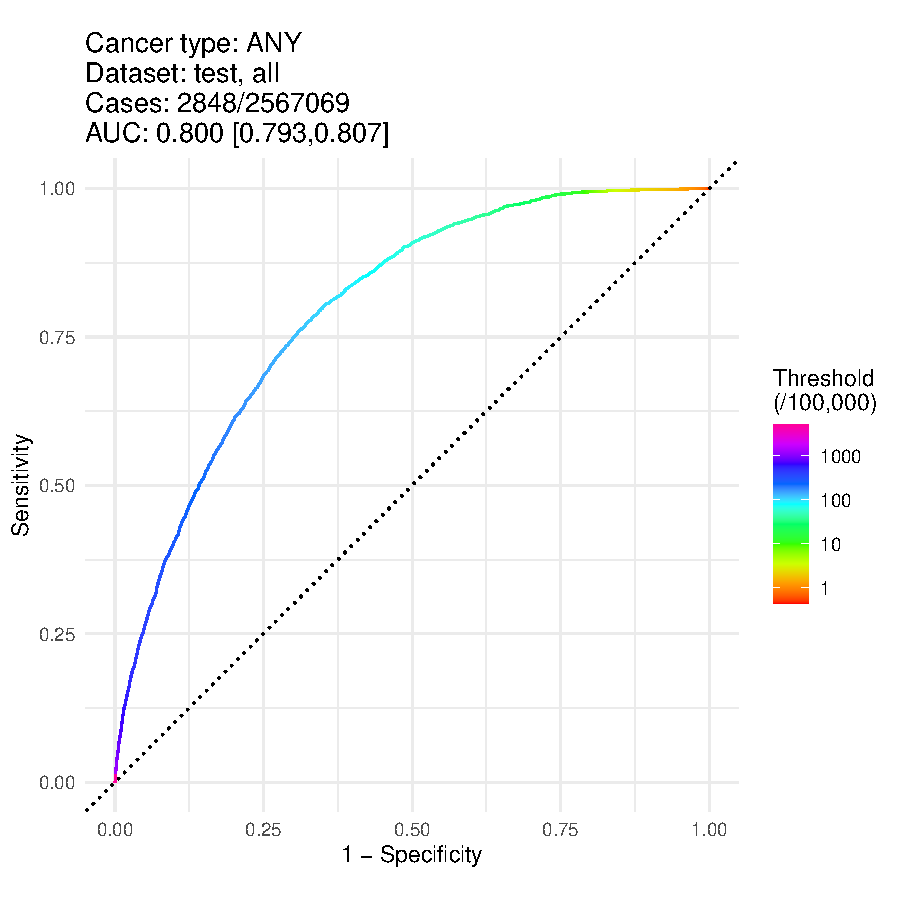
\includegraphics[width=1.0\linewidth]{roc/ANY_all.pdf}
\end{figure}
\begin{figure}[ht]
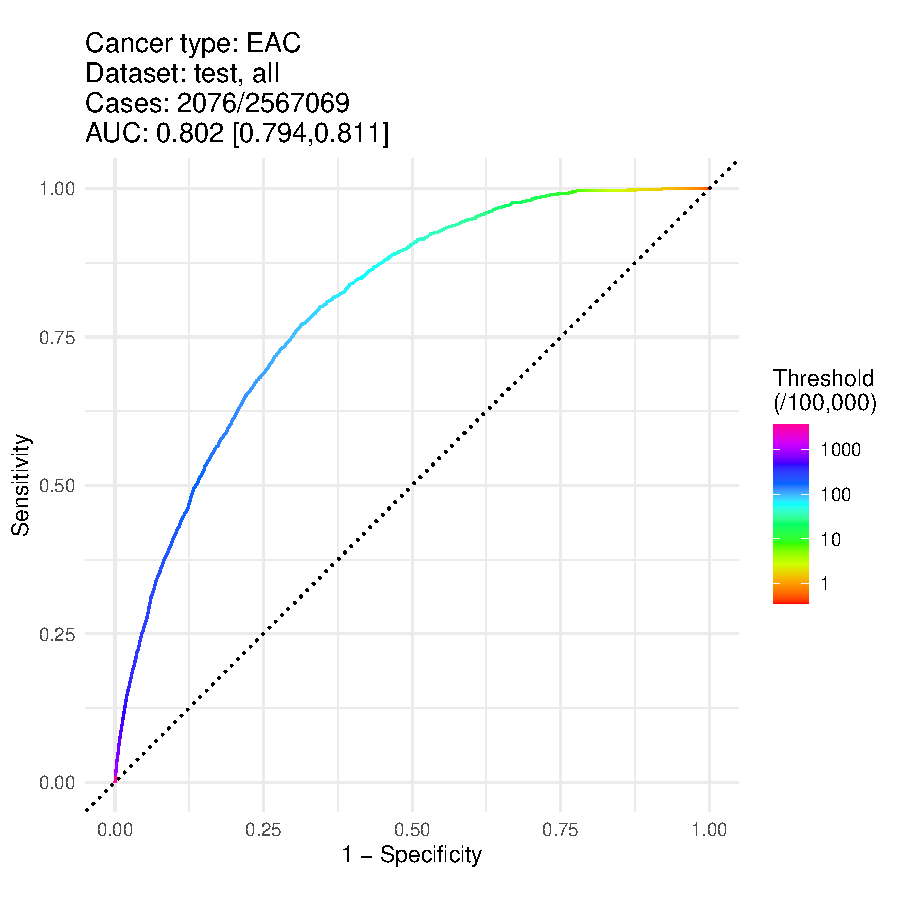
\includegraphics[width=1.0\linewidth]{roc/EAC_all.pdf}
\end{figure}
\begin{figure}[ht]
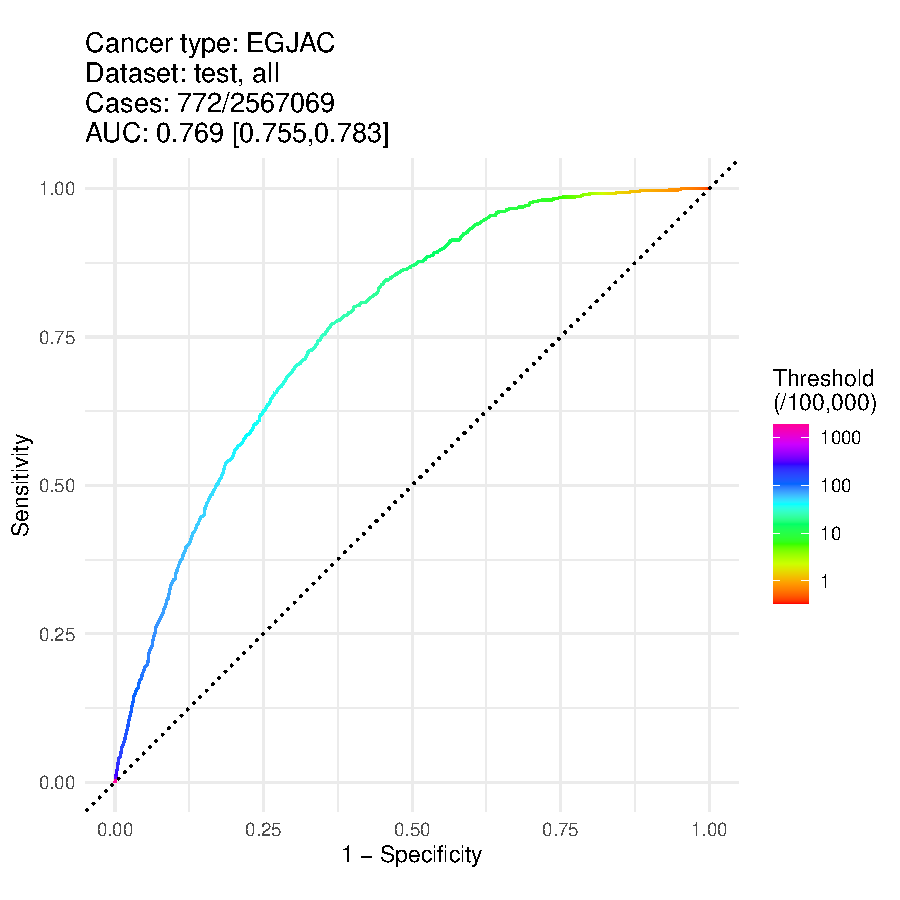
\includegraphics[width=1.0\linewidth]{roc/EGJAC_all.pdf}
\end{figure}




\newpage
\clearpage
\section{Comparison to HUNT, Kunzmann and Guidelines}

\subsection{Full test data}

\begin{figure}[ht]
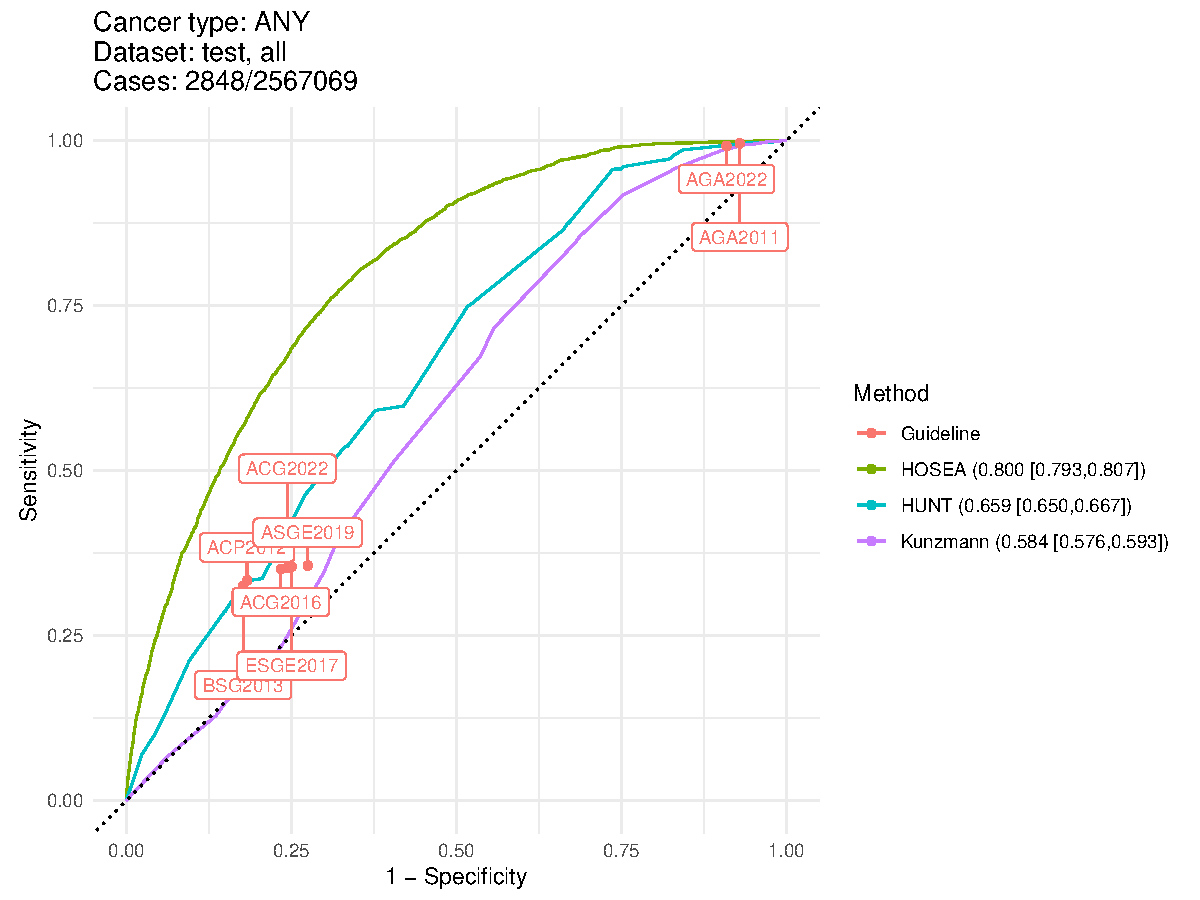
\includegraphics[width=1.0\linewidth]{comparison/ANY_all.pdf}
\end{figure}
\begin{figure}[ht]
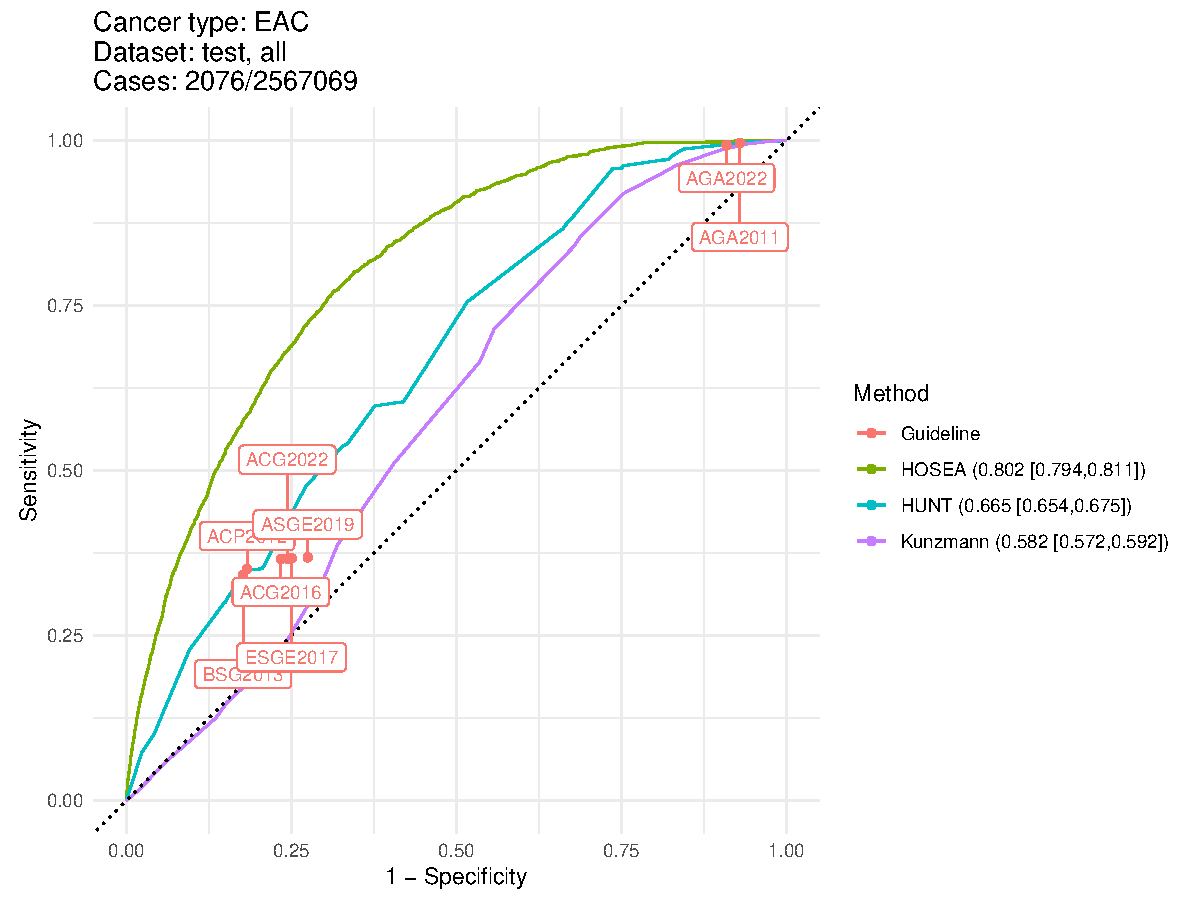
\includegraphics[width=1.0\linewidth]{comparison/EAC_all.pdf}
\end{figure}
\begin{figure}[ht]
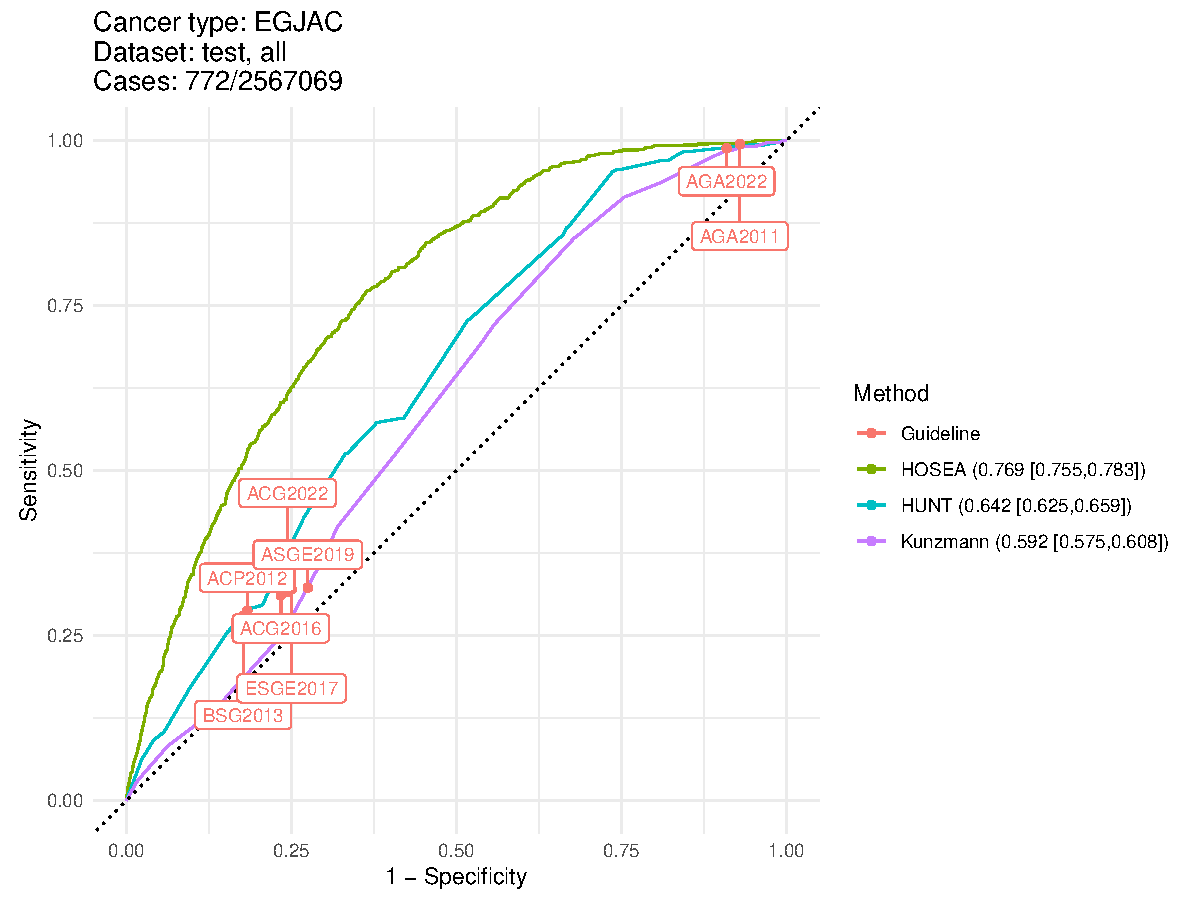
\includegraphics[width=1.0\linewidth]{comparison/EGJAC_all.pdf}
\end{figure}

\newpage
\clearpage
\subsection{Complete test patients}
\textit{w.r.t. HUNT, Kunzmann, \& Guidelines (i.e., requires age, sex, GERD, bmi, smoking, etc.)}

\begin{figure}[ht]
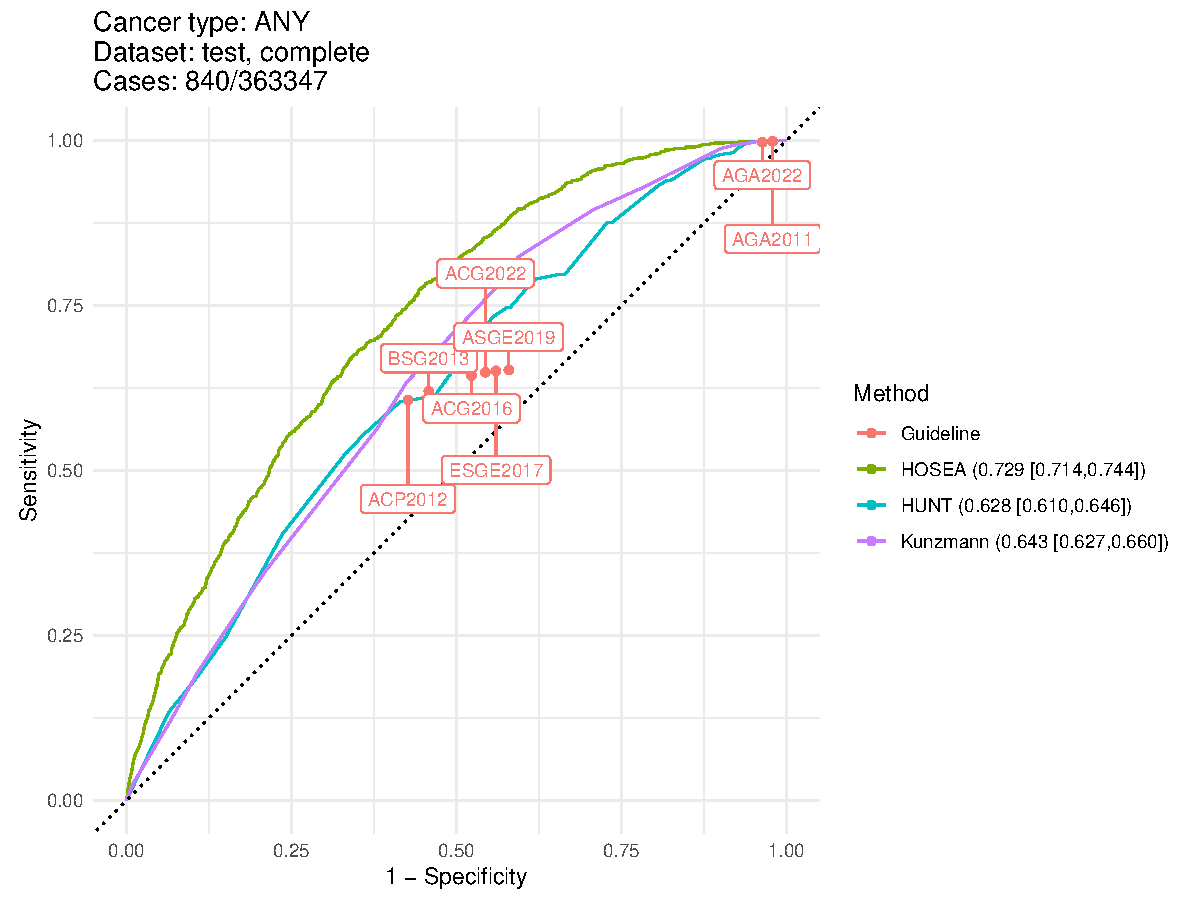
\includegraphics[width=1.0\linewidth]{comparison/ANY_complete.pdf}
\end{figure}
\begin{figure}[ht]
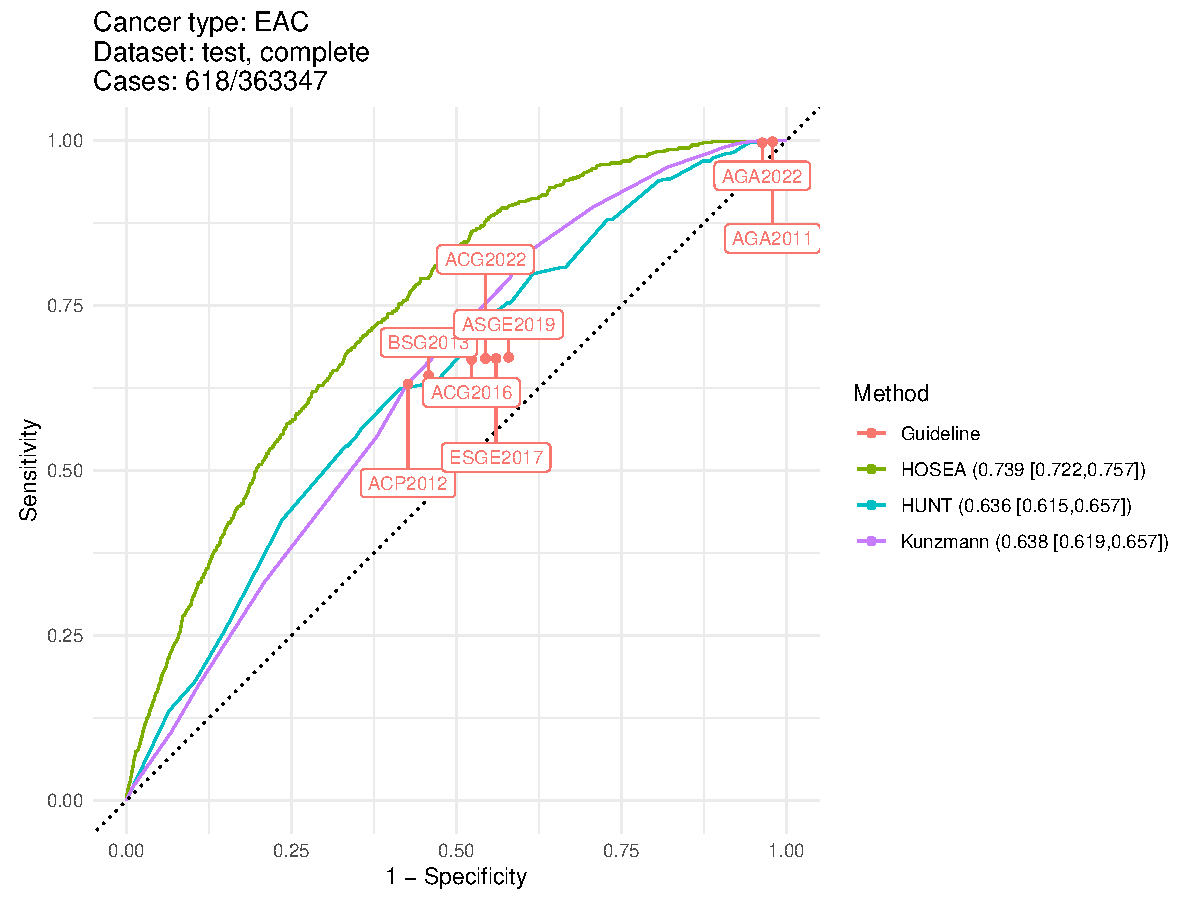
\includegraphics[width=1.0\linewidth]{comparison/EAC_complete.pdf}
\end{figure}
\begin{figure}[ht]
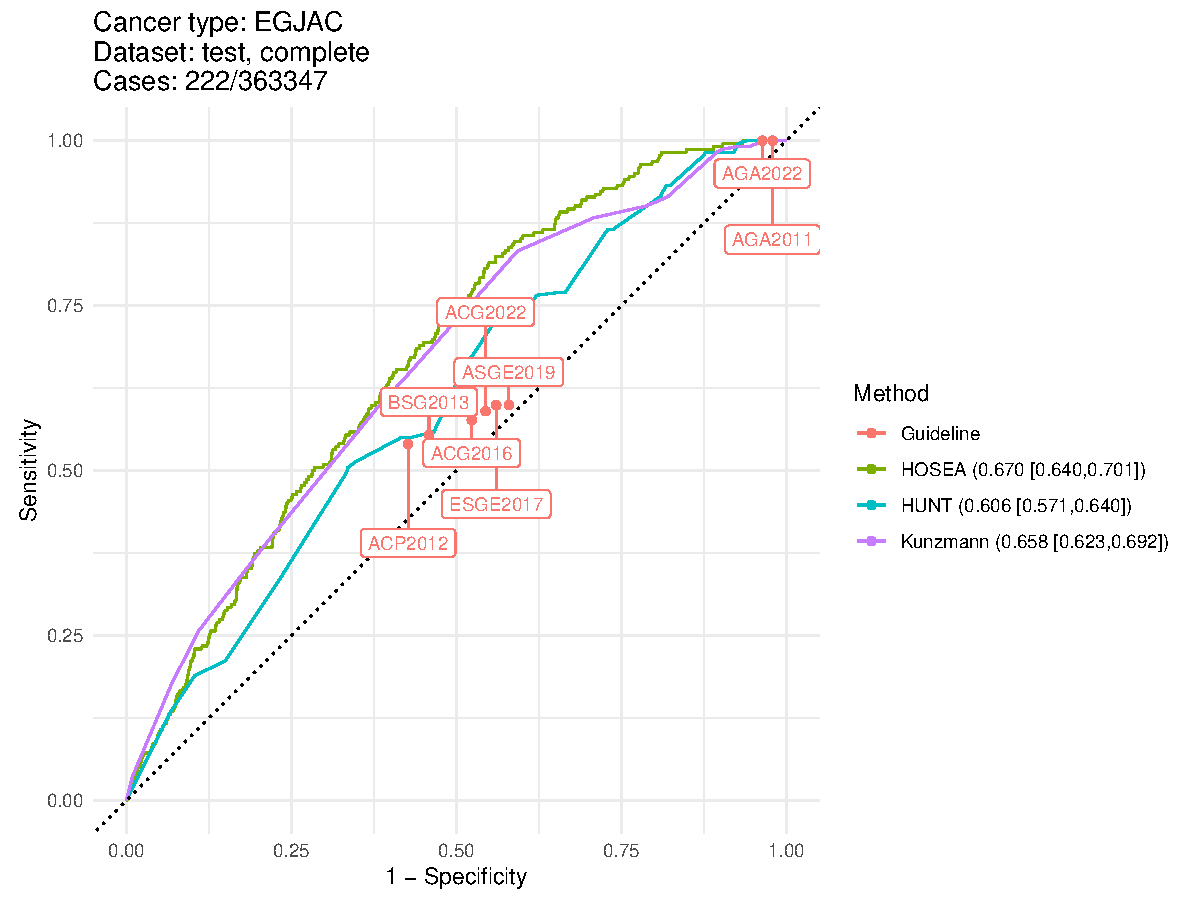
\includegraphics[width=1.0\linewidth]{comparison/EGJAC_complete.pdf}
\end{figure}


\newpage
\clearpage
\subsection{Representative sample}
\textit{w.r.t. sex and prevalance ratio by sex}

\begin{figure}[ht]
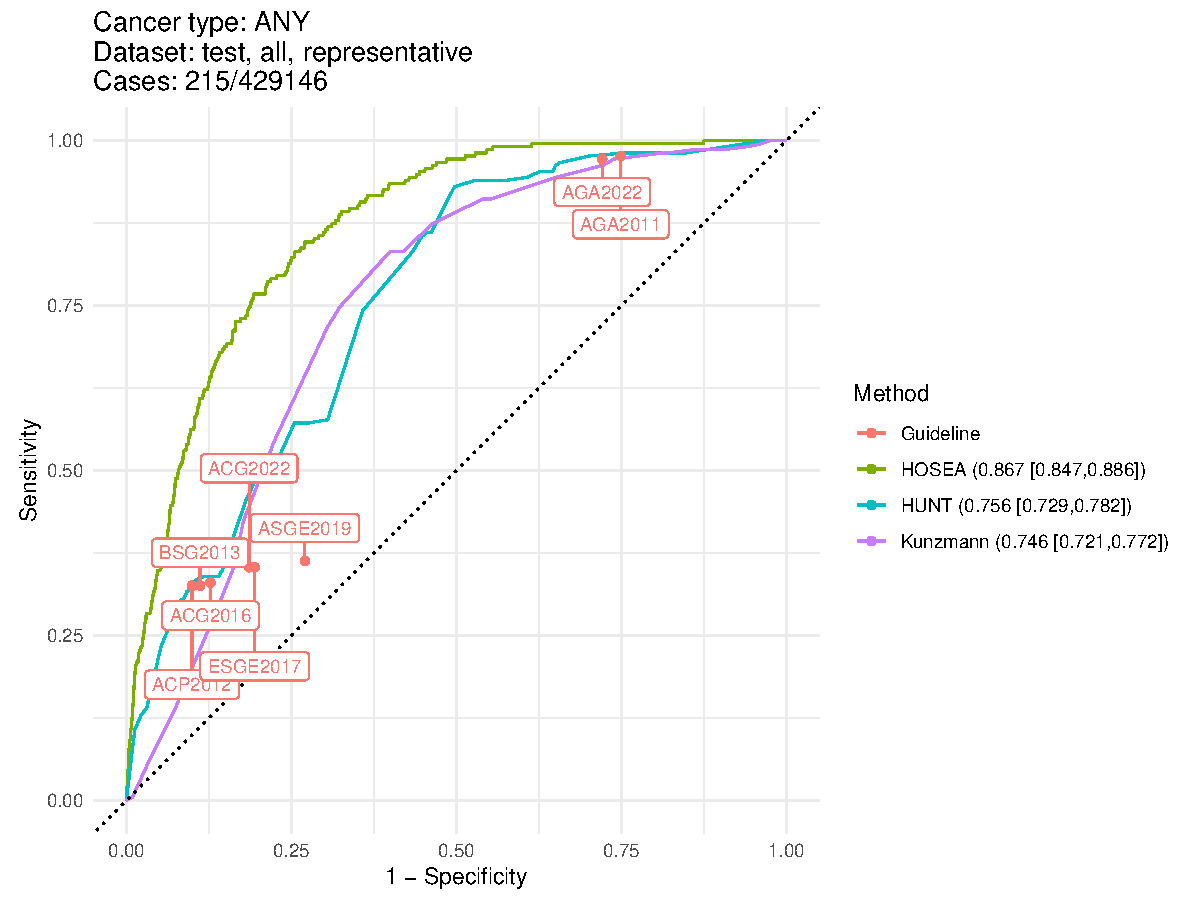
\includegraphics[width=1.0\linewidth]{comparison/ANY_all_representative.pdf}
\end{figure}
\begin{figure}[ht]
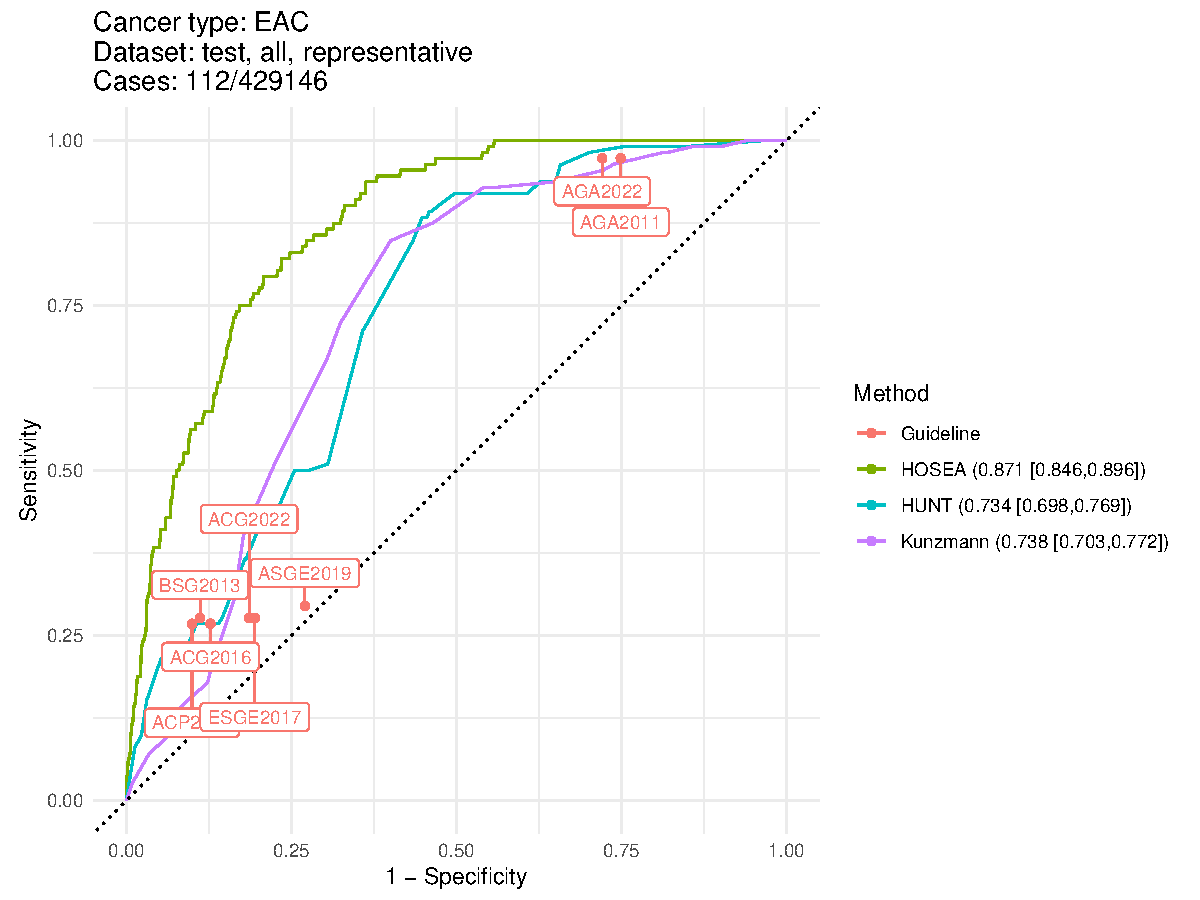
\includegraphics[width=1.0\linewidth]{comparison/EAC_all_representative.pdf}
\end{figure}
\begin{figure}[ht]
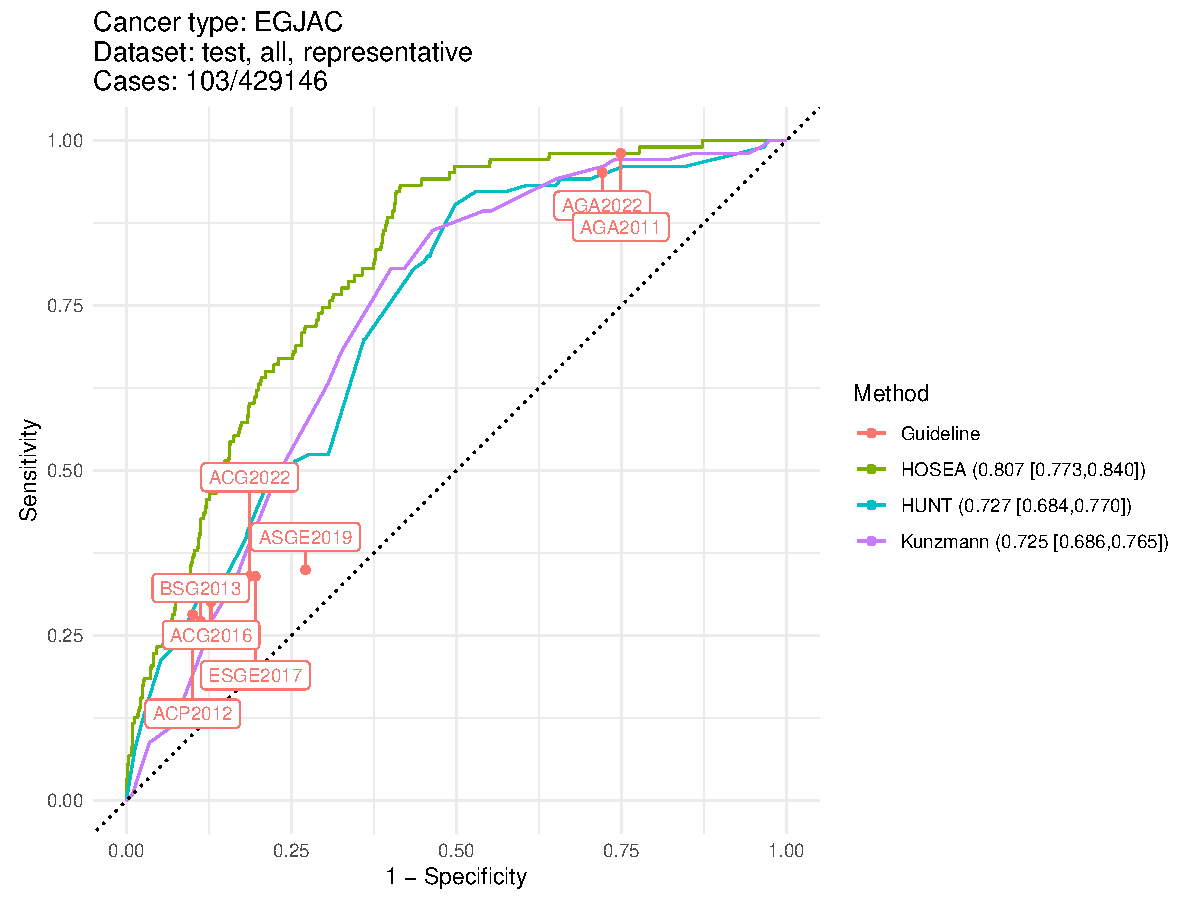
\includegraphics[width=1.0\linewidth]{comparison/EGJAC_all_representative.pdf}
\end{figure}




\newpage
\clearpage
\section{Calibration}




\begin{figure}[ht]
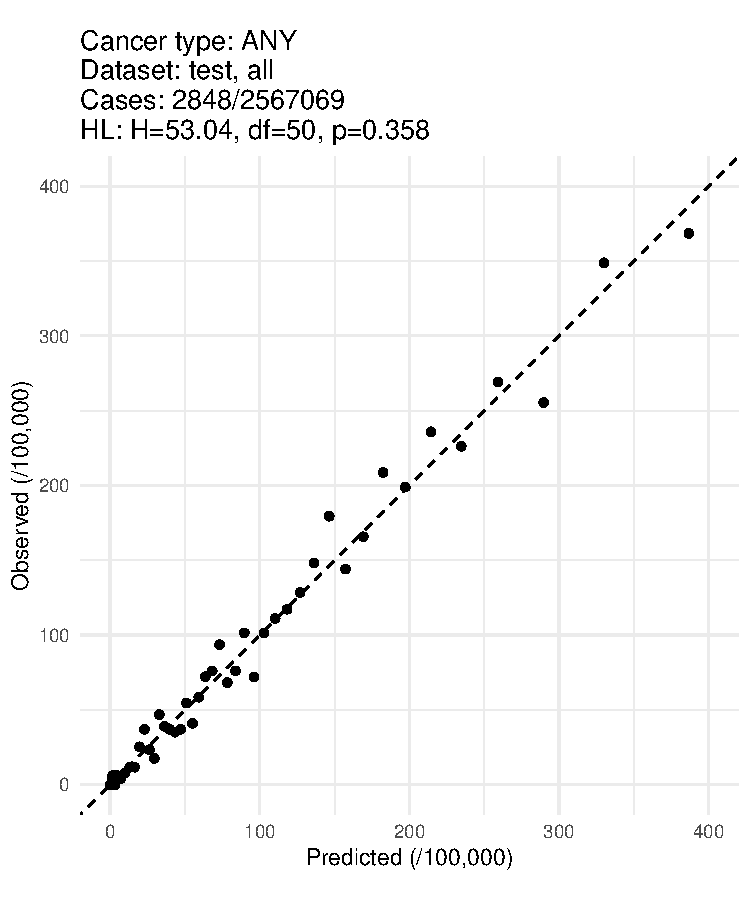
\includegraphics[width=0.9\linewidth]{calibration/ANY_all.pdf}
\end{figure}
\begin{figure}[ht]
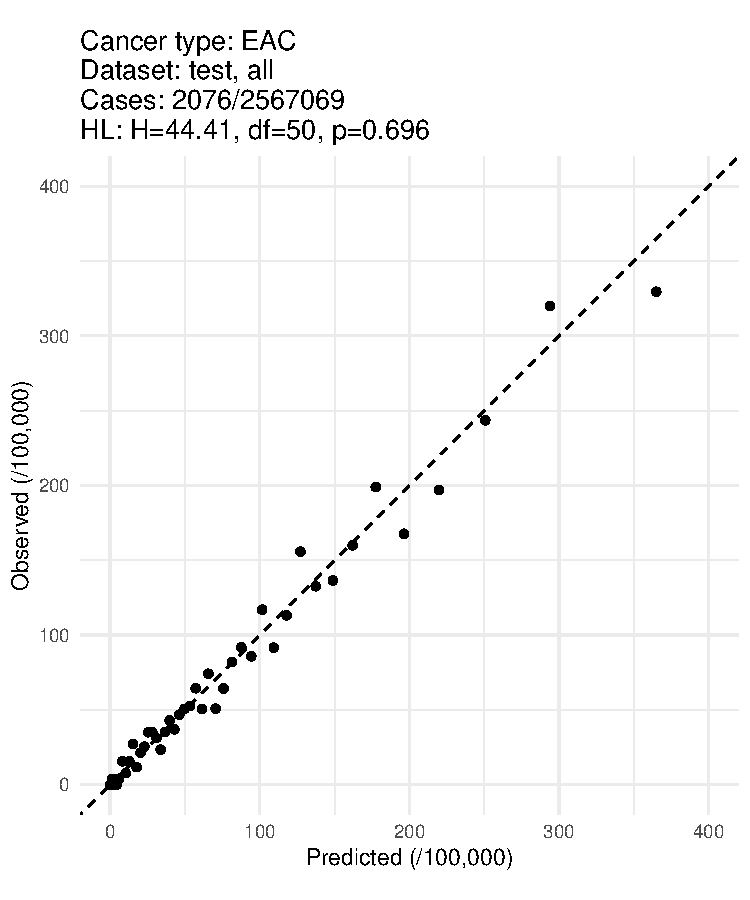
\includegraphics[width=0.9\linewidth]{calibration/EAC_all.pdf}
\end{figure}
\begin{figure}[ht]
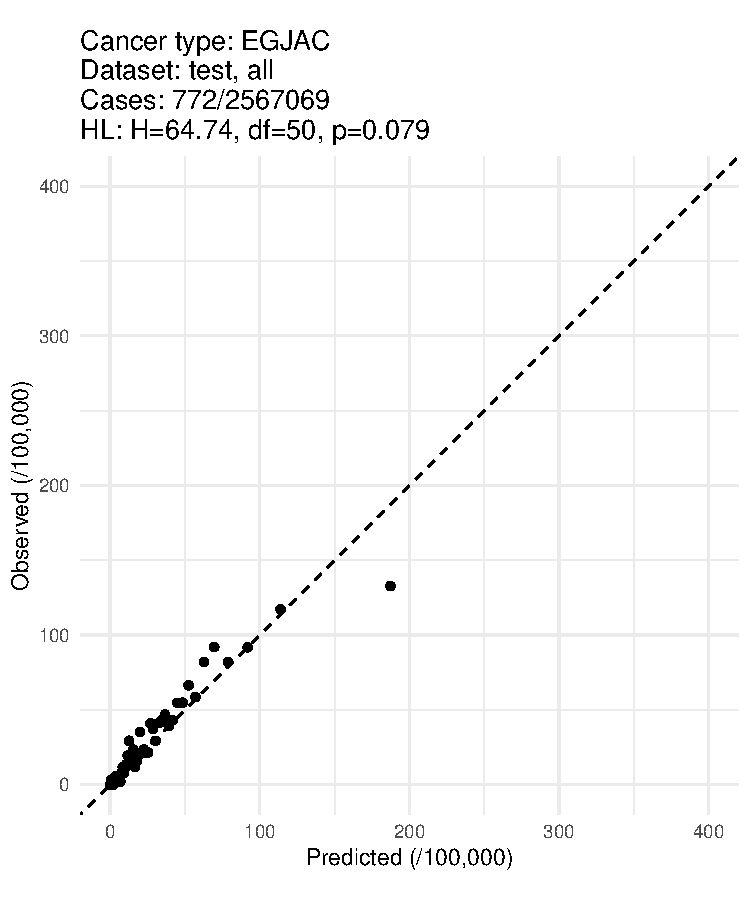
\includegraphics[width=0.9\linewidth]{calibration/EGJAC_all.pdf}
\end{figure}



\newpage
\clearpage
\section{Thresholds}

% latex table generated in R 4.2.0 by xtable 1.8-4 package
% Mon Sep 19 12:04:05 2022
\begin{table}[ht]
\centering\scriptsize
\begin{tabular}{lccc}
  \toprule
  \multicolumn{4}{l}{\textbf{ANY}}\\
Threshold & TPR & PPV & DetPrevalence \\ 
  \midrule
0 & 100.00 & 0.11 & 100.00 \\ 
  5 & 99.54 & 0.13 & 82.38 \\ 
  10 & 99.40 & 0.14 & 78.88 \\ 
  15 & 99.09 & 0.15 & 75.76 \\ 
  20 & 98.60 & 0.15 & 72.73 \\ 
   \addlinespace
25 & 97.68 & 0.16 & 69.71 \\ 
  30 & 97.16 & 0.16 & 66.67 \\ 
  35 & 96.10 & 0.17 & 63.70 \\ 
  40 & 95.19 & 0.17 & 60.83 \\ 
  45 & 94.24 & 0.18 & 58.08 \\ 
   \addlinespace
50 & 93.22 & 0.19 & 55.47 \\ 
  55 & 92.17 & 0.19 & 52.98 \\ 
  60 & 91.12 & 0.20 & 50.60 \\ 
  65 & 89.68 & 0.21 & 48.36 \\ 
  70 & 88.24 & 0.21 & 46.22 \\ 
   \addlinespace
75 & 86.73 & 0.22 & 44.21 \\ 
  80 & 85.32 & 0.22 & 42.32 \\ 
  85 & 84.23 & 0.23 & 40.53 \\ 
  90 & 82.94 & 0.24 & 38.87 \\ 
  95 & 81.64 & 0.24 & 37.30 \\ 
   \addlinespace
100 & 80.65 & 0.25 & 35.81 \\ 
  105 & 79.39 & 0.26 & 34.39 \\ 
  110 & 77.98 & 0.26 & 33.06 \\ 
  115 & 76.65 & 0.27 & 31.78 \\ 
  120 & 75.42 & 0.27 & 30.57 \\ 
   \addlinespace
125 & 73.98 & 0.28 & 29.41 \\ 
  130 & 72.75 & 0.29 & 28.30 \\ 
  135 & 71.52 & 0.29 & 27.24 \\ 
  140 & 70.19 & 0.30 & 26.23 \\ 
  145 & 68.71 & 0.30 & 25.24 \\ 
   \addlinespace
150 & 67.10 & 0.31 & 24.30 \\ 
  155 & 65.77 & 0.31 & 23.39 \\ 
  160 & 64.64 & 0.32 & 22.51 \\ 
  165 & 63.38 & 0.32 & 21.66 \\ 
  170 & 62.08 & 0.33 & 20.85 \\ 
   \addlinespace
175 & 61.17 & 0.34 & 20.07 \\ 
  180 & 59.59 & 0.34 & 19.33 \\ 
  185 & 58.39 & 0.35 & 18.61 \\ 
  190 & 57.09 & 0.35 & 17.93 \\ 
  195 & 56.04 & 0.36 & 17.27 \\ 
   \addlinespace
200 & 54.95 & 0.37 & 16.64 \\ 
  220 & 50.49 & 0.39 & 14.38 \\ 
  240 & 46.52 & 0.41 & 12.50 \\ 
  260 & 42.84 & 0.44 & 10.92 \\ 
  280 & 39.54 & 0.46 & 9.56 \\ 
   \addlinespace
300 & 37.18 & 0.49 & 8.40 \\ 
  320 & 34.02 & 0.51 & 7.41 \\ 
  340 & 31.07 & 0.53 & 6.56 \\ 
  360 & 29.14 & 0.56 & 5.81 \\ 
  380 & 26.83 & 0.58 & 5.16 \\ 
   \addlinespace
400 & 24.72 & 0.60 & 4.59 \\ 
  420 & 23.24 & 0.63 & 4.09 \\ 
  440 & 21.38 & 0.65 & 3.65 \\ 
  460 & 19.73 & 0.67 & 3.26 \\ 
  480 & 18.64 & 0.71 & 2.92 \\ 
   \addlinespace
500 & 17.38 & 0.74 & 2.62 \\ 
  550 & 14.54 & 0.81 & 2.00 \\ 
  600 & 12.46 & 0.90 & 1.53 \\ 
  650 & 10.29 & 0.96 & 1.19 \\ 
  700 & 8.25 & 0.98 & 0.93 \\ 
   \addlinespace
750 & 7.16 & 1.08 & 0.73 \\ 
  800 & 5.76 & 1.09 & 0.58 \\ 
  850 & 4.88 & 1.16 & 0.47 \\ 
  900 & 4.39 & 1.30 & 0.37 \\ 
  950 & 3.79 & 1.38 & 0.31 \\ 
   \addlinespace
1000 & 3.41 & 1.52 & 0.25 \\ 
   \bottomrule
\end{tabular}
\end{table}

% latex table generated in R 4.2.0 by xtable 1.8-4 package
% Mon Sep 19 12:11:22 2022
\begin{table}[ht]
\centering\scriptsize
\begin{tabular}{lccc}
  \toprule
  \multicolumn{4}{l}{\textbf{EAC}}\\
Threshold & TPR & PPV & DetPrevalence \\ 
  \midrule
0 & 100.00 & 0.08 & 100.00 \\ 
  5 & 99.71 & 0.10 & 79.96 \\ 
  10 & 99.18 & 0.11 & 75.25 \\ 
  15 & 98.55 & 0.11 & 71.17 \\ 
  20 & 97.59 & 0.12 & 67.18 \\ 
   \addlinespace
25 & 96.15 & 0.12 & 63.30 \\ 
  30 & 94.75 & 0.13 & 59.59 \\ 
  35 & 93.55 & 0.13 & 56.09 \\ 
  40 & 92.05 & 0.14 & 52.76 \\ 
  45 & 90.37 & 0.15 & 49.65 \\ 
   \addlinespace
50 & 88.87 & 0.15 & 46.76 \\ 
  55 & 86.95 & 0.16 & 44.05 \\ 
  60 & 84.97 & 0.17 & 41.56 \\ 
  65 & 83.33 & 0.17 & 39.26 \\ 
  70 & 81.79 & 0.18 & 37.16 \\ 
   \addlinespace
75 & 80.39 & 0.18 & 35.24 \\ 
  80 & 78.85 & 0.19 & 33.45 \\ 
  85 & 77.31 & 0.20 & 31.80 \\ 
  90 & 75.53 & 0.20 & 30.23 \\ 
  95 & 73.70 & 0.21 & 28.77 \\ 
   \addlinespace
100 & 72.11 & 0.21 & 27.39 \\ 
  105 & 70.42 & 0.22 & 26.08 \\ 
  110 & 68.64 & 0.22 & 24.82 \\ 
  115 & 67.29 & 0.23 & 23.63 \\ 
  120 & 65.70 & 0.24 & 22.50 \\ 
   \addlinespace
125 & 64.07 & 0.24 & 21.43 \\ 
  130 & 62.19 & 0.25 & 20.41 \\ 
  135 & 60.16 & 0.25 & 19.43 \\ 
  140 & 58.67 & 0.26 & 18.50 \\ 
  145 & 57.42 & 0.26 & 17.62 \\ 
   \addlinespace
150 & 56.02 & 0.27 & 16.78 \\ 
  155 & 54.62 & 0.28 & 16.00 \\ 
  160 & 53.42 & 0.28 & 15.27 \\ 
  165 & 51.73 & 0.29 & 14.57 \\ 
  170 & 50.43 & 0.29 & 13.90 \\ 
   \addlinespace
175 & 49.37 & 0.30 & 13.27 \\ 
  180 & 47.54 & 0.30 & 12.69 \\ 
  185 & 45.86 & 0.31 & 12.13 \\ 
  190 & 44.89 & 0.31 & 11.61 \\ 
  195 & 43.93 & 0.32 & 11.10 \\ 
   \addlinespace
200 & 42.82 & 0.33 & 10.62 \\ 
  220 & 38.97 & 0.35 & 8.96 \\ 
  240 & 35.50 & 0.38 & 7.59 \\ 
  260 & 32.23 & 0.40 & 6.47 \\ 
  280 & 28.37 & 0.42 & 5.52 \\ 
   \addlinespace
300 & 25.72 & 0.44 & 4.74 \\ 
  320 & 23.03 & 0.46 & 4.08 \\ 
  340 & 20.86 & 0.48 & 3.52 \\ 
  360 & 19.08 & 0.51 & 3.04 \\ 
  380 & 17.15 & 0.53 & 2.64 \\ 
   \addlinespace
400 & 15.90 & 0.56 & 2.29 \\ 
  420 & 14.60 & 0.59 & 1.99 \\ 
  440 & 12.96 & 0.60 & 1.73 \\ 
  460 & 11.85 & 0.63 & 1.52 \\ 
  480 & 10.69 & 0.65 & 1.33 \\ 
   \addlinespace
500 & 9.78 & 0.68 & 1.16 \\ 
  550 & 7.66 & 0.73 & 0.85 \\ 
  600 & 5.92 & 0.77 & 0.62 \\ 
  650 & 4.53 & 0.79 & 0.47 \\ 
  700 & 3.85 & 0.90 & 0.35 \\ 
   \addlinespace
750 & 3.32 & 1.01 & 0.27 \\ 
  800 & 2.46 & 0.98 & 0.20 \\ 
  850 & 1.83 & 0.95 & 0.16 \\ 
  900 & 1.49 & 1.01 & 0.12 \\ 
  950 & 1.25 & 1.08 & 0.09 \\ 
   \addlinespace
1000 & 1.16 & 1.27 & 0.07 \\ 
   \bottomrule
\end{tabular}
\end{table}

% latex table generated in R 4.2.0 by xtable 1.8-4 package
% Mon Sep 19 12:18:46 2022
\begin{table}[ht]
\centering\scriptsize
\begin{tabular}{lccc}
  \toprule
  \multicolumn{4}{l}{\textbf{EGJAC}}\\
Threshold & TPR & PPV & DetPrevalence \\ 
  \midrule
0 & 100.00 & 0.03 & 100.00 \\ 
  5 & 98.58 & 0.04 & 76.82 \\ 
  10 & 96.11 & 0.04 & 65.06 \\ 
  15 & 89.25 & 0.05 & 53.93 \\ 
  20 & 83.68 & 0.06 & 44.85 \\ 
   \addlinespace
25 & 77.72 & 0.06 & 37.42 \\ 
  30 & 70.85 & 0.07 & 31.35 \\ 
  35 & 64.64 & 0.07 & 26.37 \\ 
  40 & 58.55 & 0.08 & 22.29 \\ 
  45 & 53.89 & 0.09 & 18.91 \\ 
   \addlinespace
50 & 48.32 & 0.09 & 16.12 \\ 
  55 & 43.26 & 0.09 & 13.78 \\ 
  60 & 38.99 & 0.10 & 11.84 \\ 
  65 & 34.97 & 0.10 & 10.23 \\ 
  70 & 30.83 & 0.10 & 8.87 \\ 
   \addlinespace
75 & 27.85 & 0.11 & 7.71 \\ 
  80 & 25.26 & 0.11 & 6.73 \\ 
  85 & 22.54 & 0.11 & 5.90 \\ 
  90 & 19.56 & 0.11 & 5.19 \\ 
  95 & 18.01 & 0.12 & 4.58 \\ 
   \addlinespace
100 & 16.84 & 0.12 & 4.06 \\ 
  105 & 15.41 & 0.13 & 3.60 \\ 
  110 & 14.51 & 0.14 & 3.20 \\ 
  115 & 12.82 & 0.14 & 2.86 \\ 
  120 & 11.40 & 0.13 & 2.55 \\ 
   \addlinespace
125 & 10.23 & 0.13 & 2.28 \\ 
  130 & 8.94 & 0.13 & 2.05 \\ 
  135 & 8.16 & 0.13 & 1.84 \\ 
  140 & 7.38 & 0.13 & 1.66 \\ 
  145 & 6.87 & 0.14 & 1.50 \\ 
   \addlinespace
150 & 6.35 & 0.14 & 1.36 \\ 
  155 & 5.96 & 0.15 & 1.23 \\ 
  160 & 5.83 & 0.16 & 1.12 \\ 
  165 & 5.05 & 0.15 & 1.02 \\ 
  170 & 4.79 & 0.16 & 0.92 \\ 
   \addlinespace
175 & 4.27 & 0.15 & 0.84 \\ 
  180 & 4.27 & 0.17 & 0.77 \\ 
  185 & 4.15 & 0.18 & 0.70 \\ 
  190 & 4.02 & 0.19 & 0.64 \\ 
  195 & 3.63 & 0.19 & 0.59 \\ 
   \addlinespace
200 & 3.37 & 0.19 & 0.54 \\ 
  220 & 2.46 & 0.19 & 0.39 \\ 
  240 & 2.07 & 0.22 & 0.28 \\ 
  260 & 1.55 & 0.22 & 0.21 \\ 
  280 & 1.17 & 0.22 & 0.16 \\ 
   \addlinespace
300 & 0.78 & 0.20 & 0.12 \\ 
  320 & 0.78 & 0.26 & 0.09 \\ 
  340 & 0.39 & 0.17 & 0.07 \\ 
  360 & 0.39 & 0.21 & 0.05 \\ 
  380 & 0.39 & 0.27 & 0.04 \\ 
   \addlinespace
400 & 0.39 & 0.34 & 0.03 \\ 
  420 & 0.13 & 0.14 & 0.03 \\ 
  440 & 0.13 & 0.18 & 0.02 \\ 
  460 & 0.13 & 0.22 & 0.02 \\ 
  480 & 0.13 & 0.28 & 0.01 \\ 
   \addlinespace
500 & 0.13 & 0.34 & 0.01 \\ 
  550 & 0.13 & 0.53 & 0.01 \\ 
  600 & 0.00 & 0.00 & 0.00 \\ 
  650 & 0.00 & 0.00 & 0.00 \\ 
  700 & 0.00 & 0.00 & 0.00 \\ 
   \addlinespace
750 & 0.00 & 0.00 & 0.00 \\ 
  800 & 0.00 & 0.00 & 0.00 \\ 
  850 & 0.00 & 0.00 & 0.00 \\ 
  900 & 0.00 & 0.00 & 0.00 \\ 
  950 & 0.00 & 0.00 & 0.00 \\ 
   \addlinespace
1000 & 0.00 & 0.00 & 0.00 \\ 
   \bottomrule
\end{tabular}
\end{table}


\newpage
\clearpage
\section{Stratification by identity groups}

\subsection{Age}

\begin{figure}[ht]
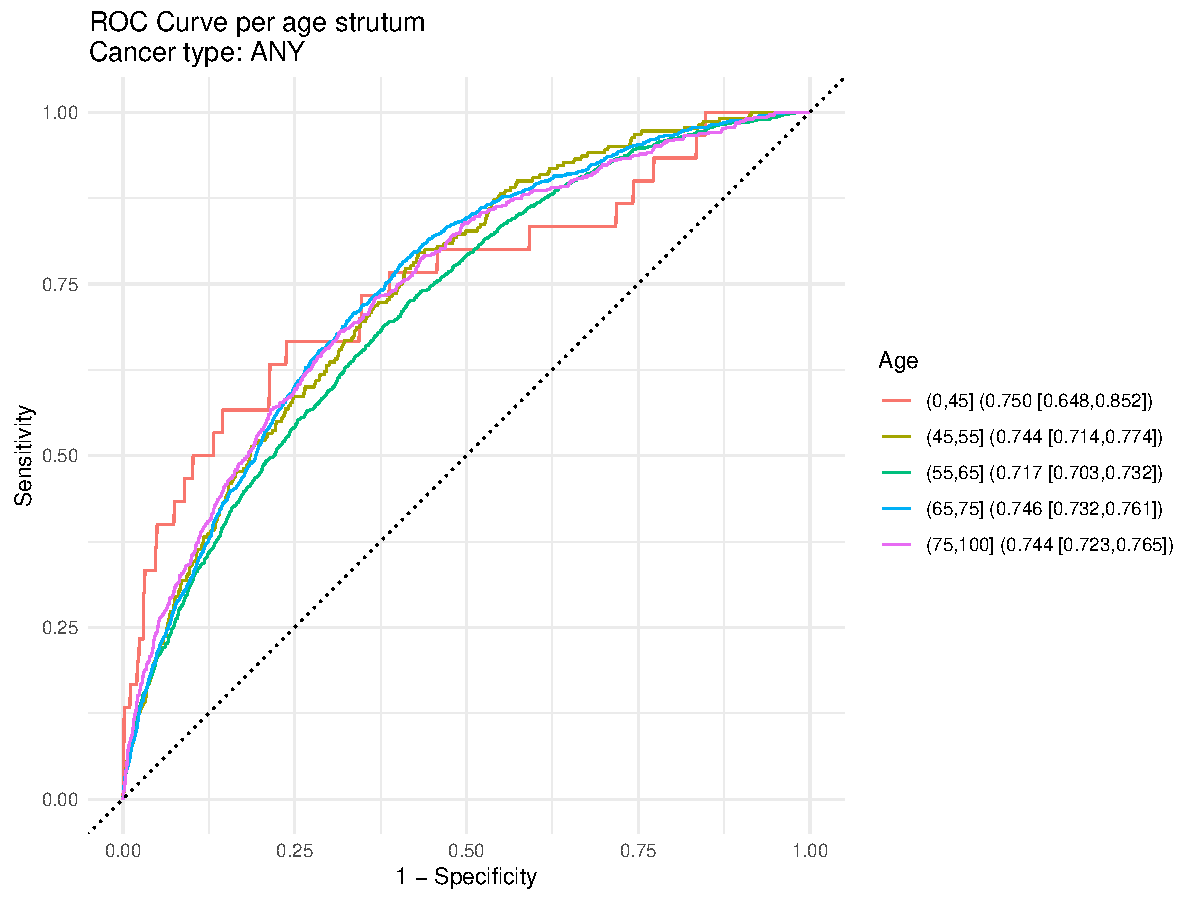
\includegraphics[width=1.0\linewidth]{identity/ANY_age.pdf}
\end{figure}
\begin{figure}[ht]
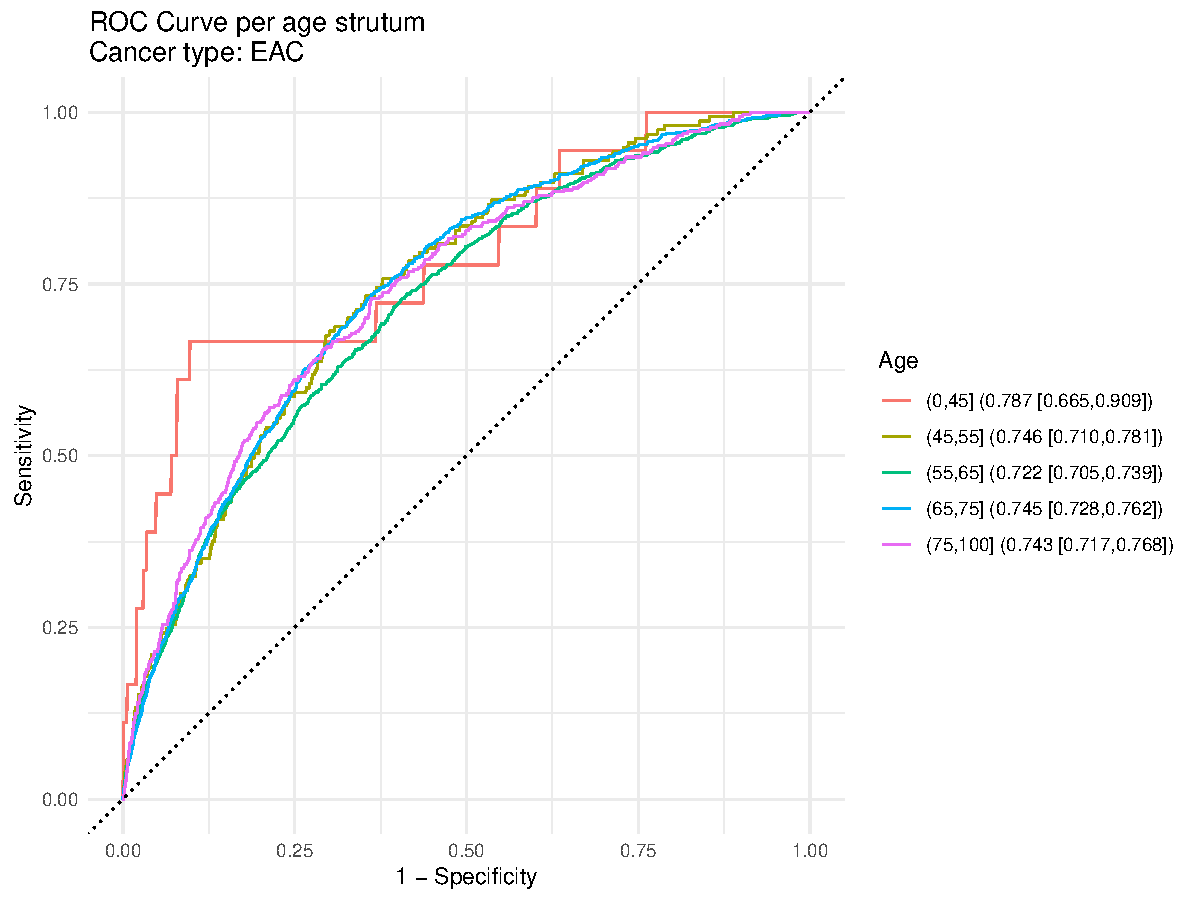
\includegraphics[width=1.0\linewidth]{identity/EAC_age.pdf}
\end{figure}
\begin{figure}[ht]
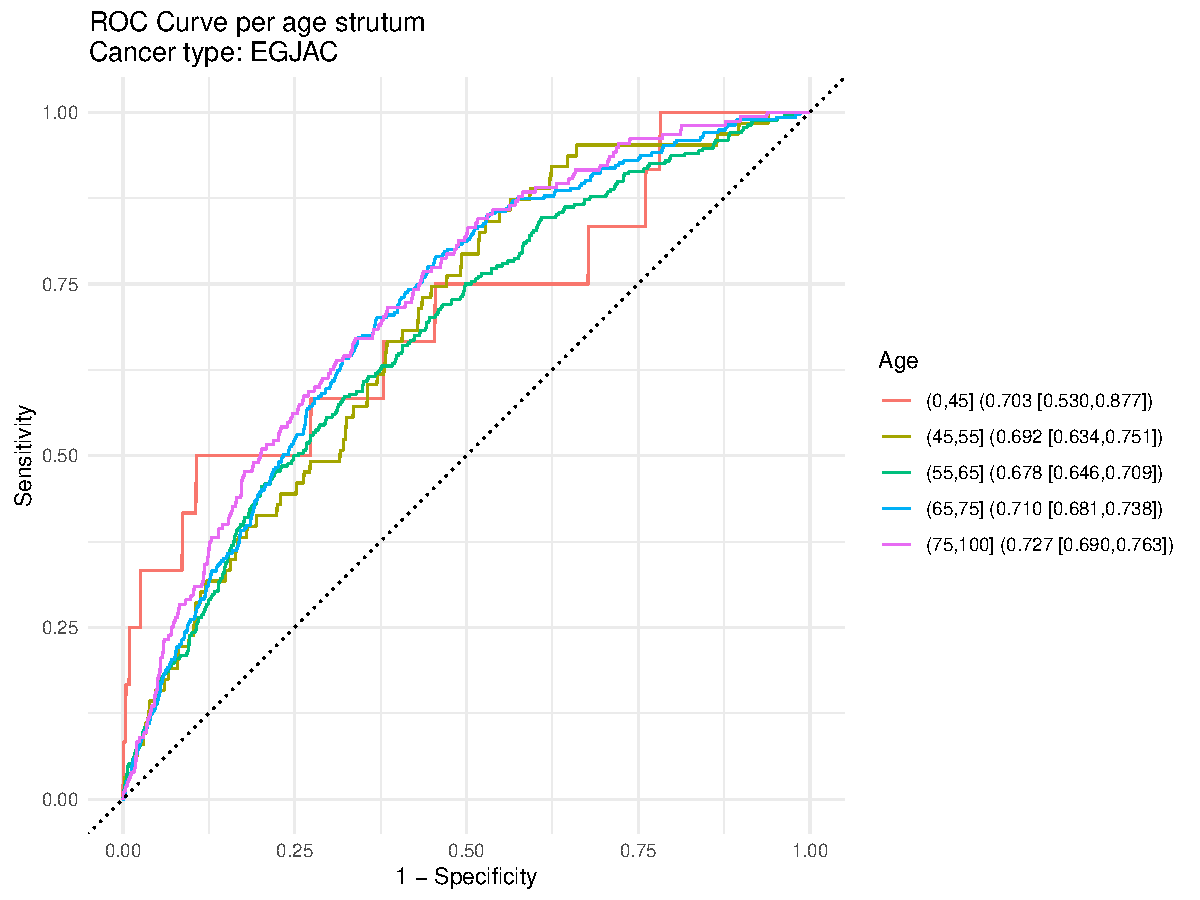
\includegraphics[width=1.0\linewidth]{identity/EGJAC_age.pdf}
\end{figure}

\newpage
\clearpage
\subsection{Sex}

\begin{figure}[ht]
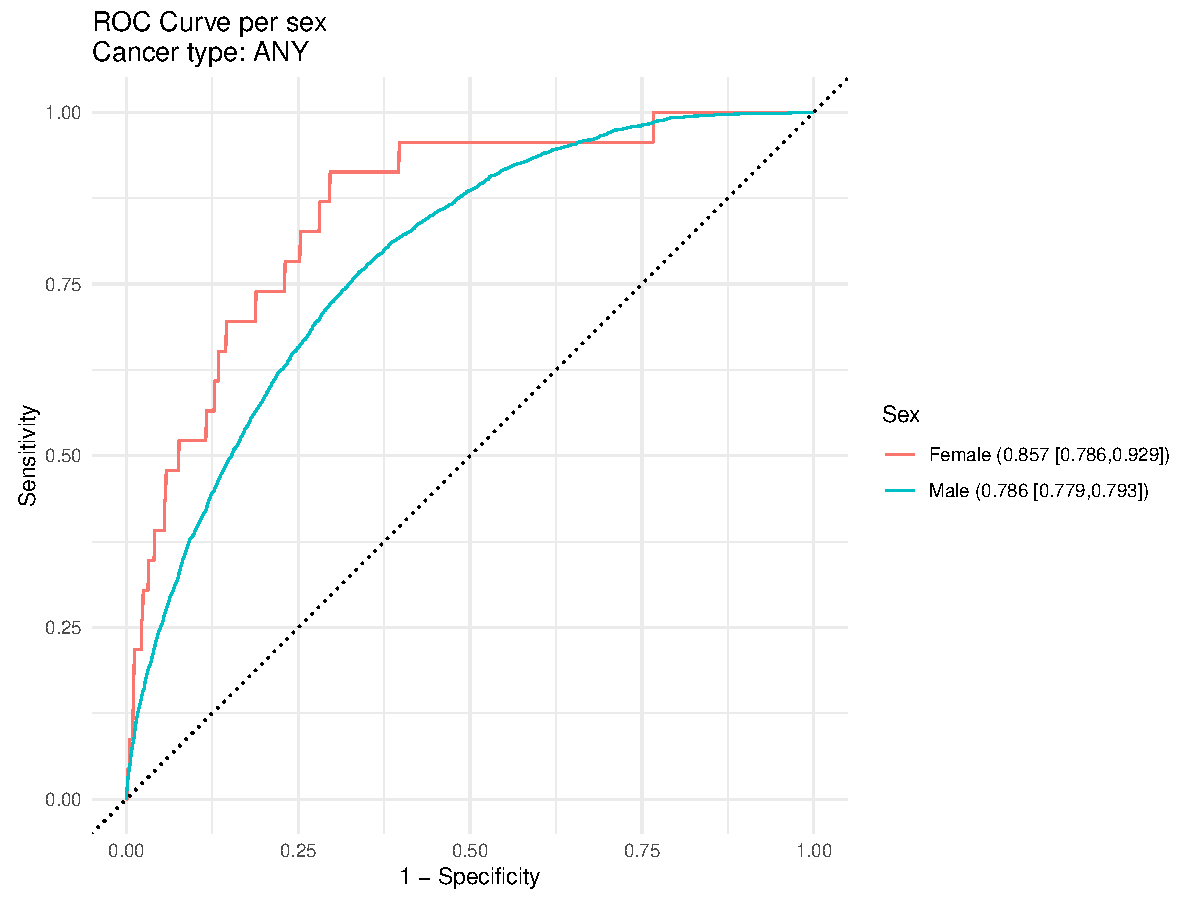
\includegraphics[width=1.0\linewidth]{identity/ANY_sex.pdf}
\end{figure}
\begin{figure}[ht]
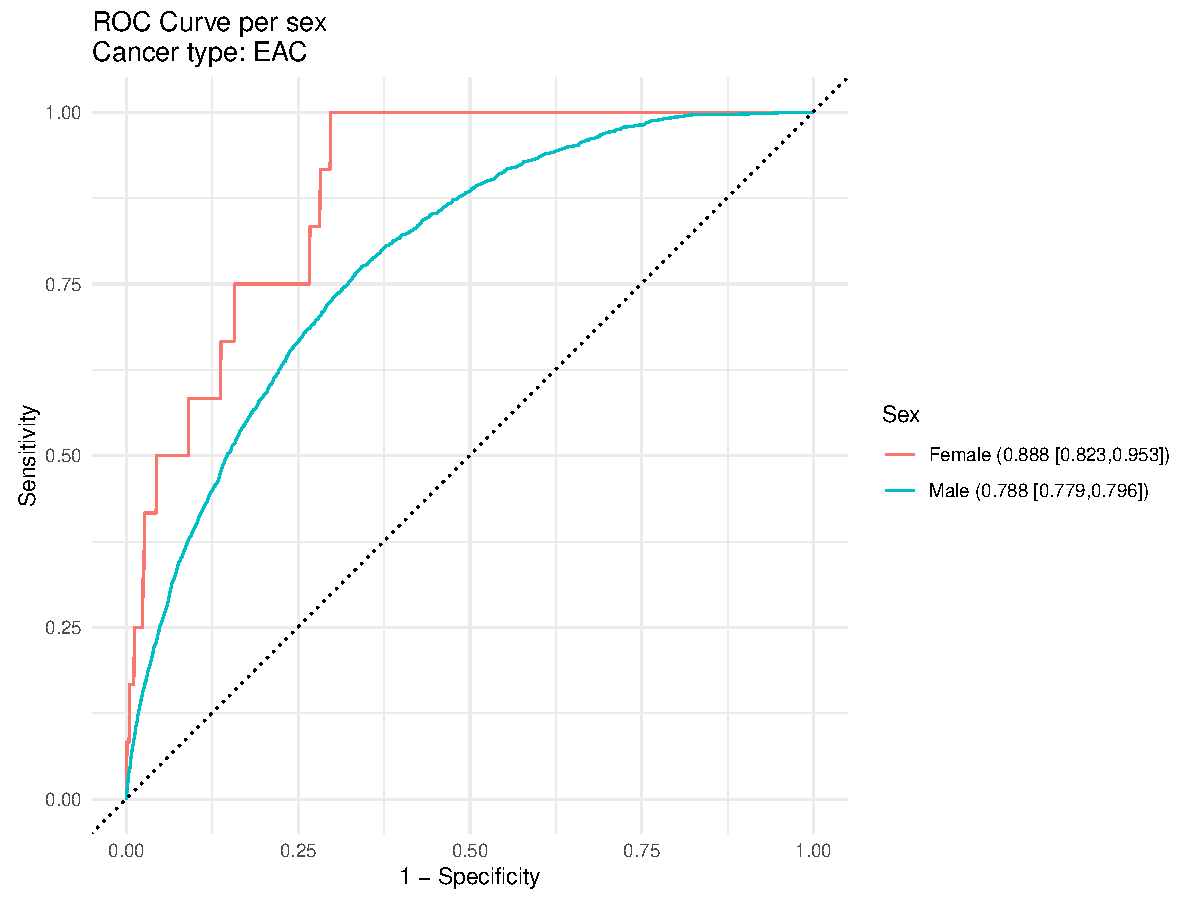
\includegraphics[width=1.0\linewidth]{identity/EAC_sex.pdf}
\end{figure}
\begin{figure}[ht]
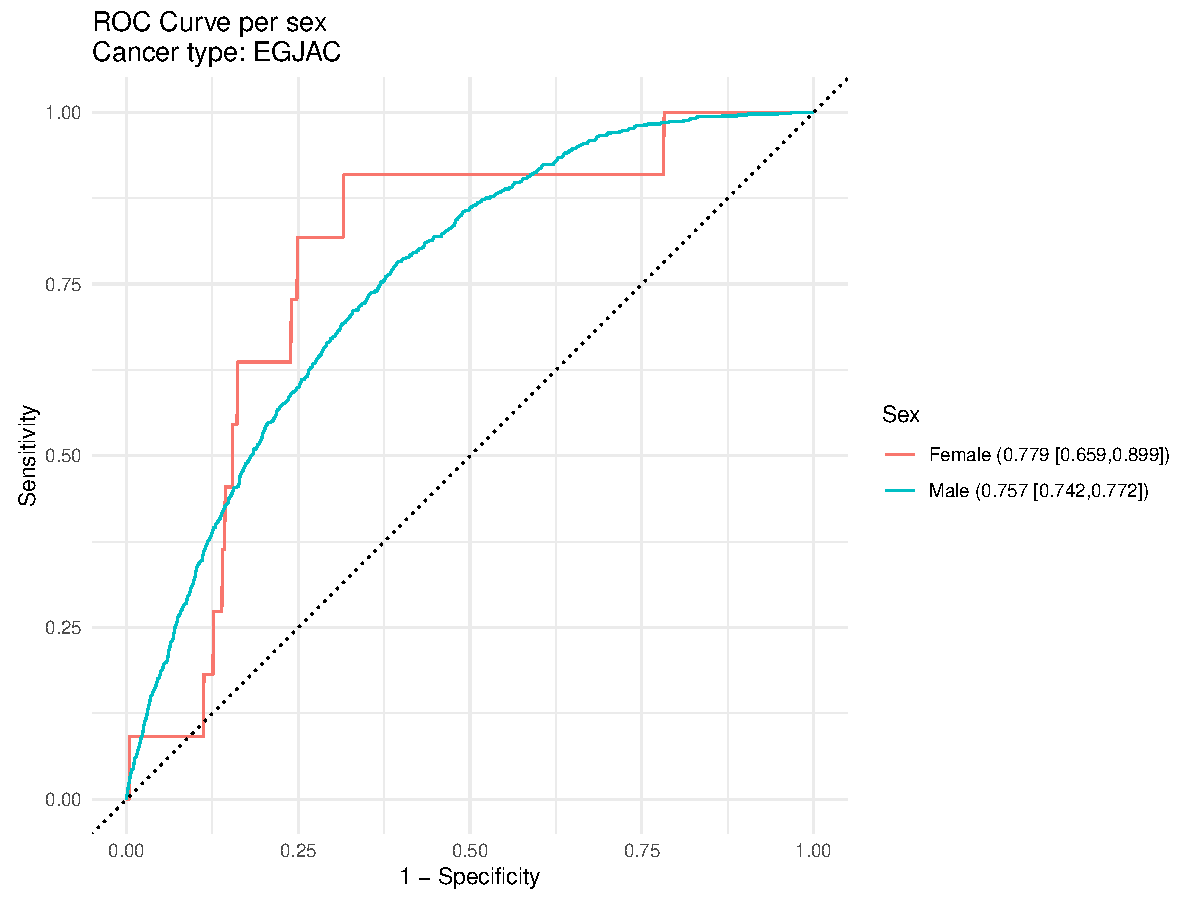
\includegraphics[width=1.0\linewidth]{identity/EGJAC_sex.pdf}
\end{figure}


\newpage
\clearpage
\subsection{Race}

\begin{figure}[ht]
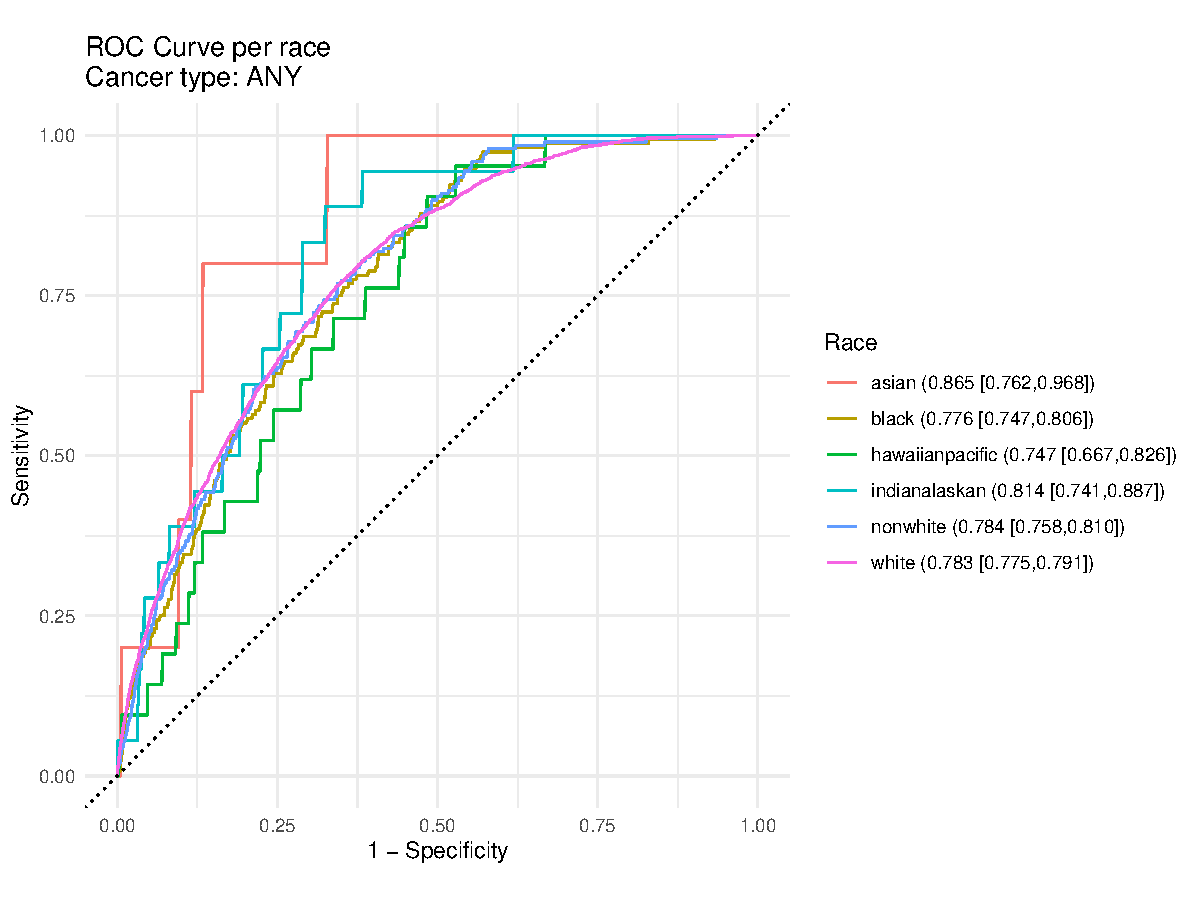
\includegraphics[width=1.0\linewidth]{identity/ANY_race.pdf}
\end{figure}
\begin{figure}[ht]
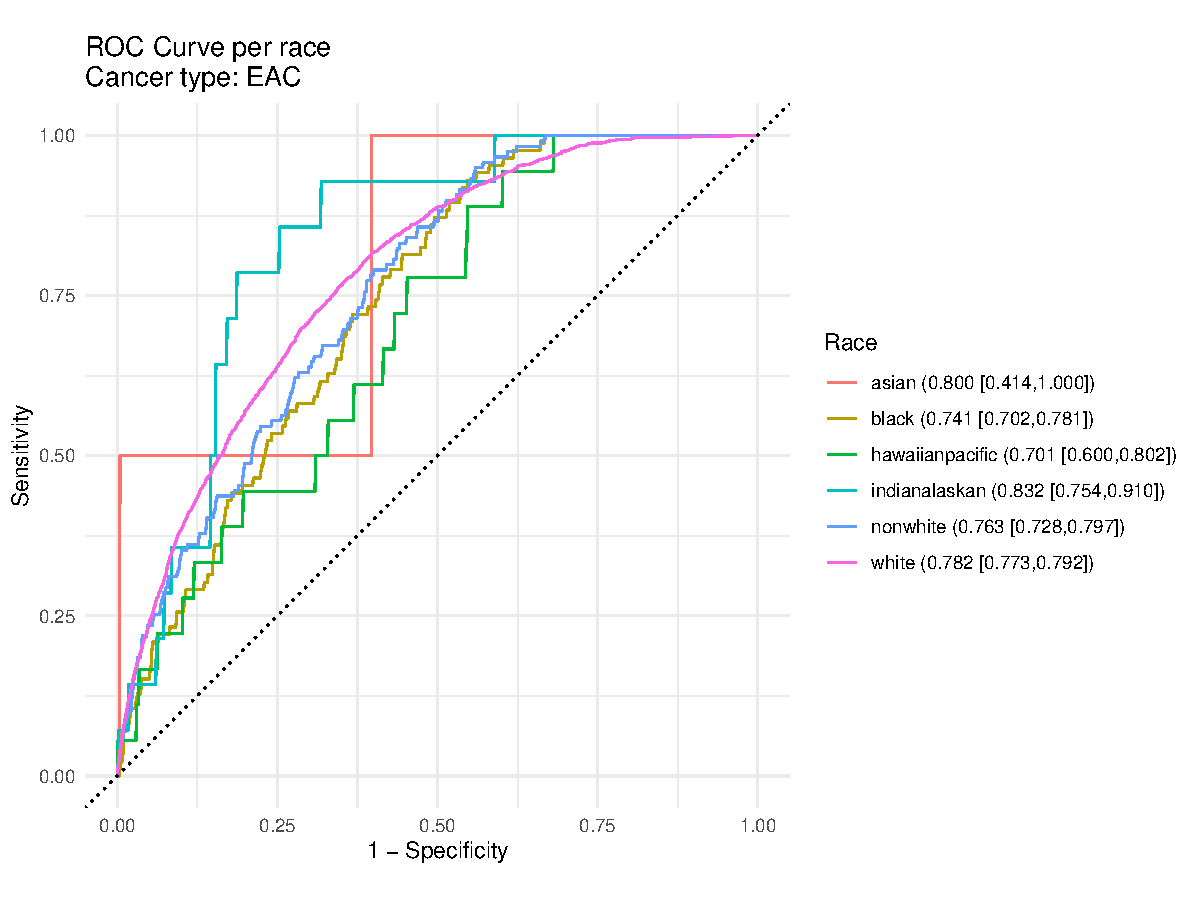
\includegraphics[width=1.0\linewidth]{identity/EAC_race.pdf}
\end{figure}
\begin{figure}[ht]
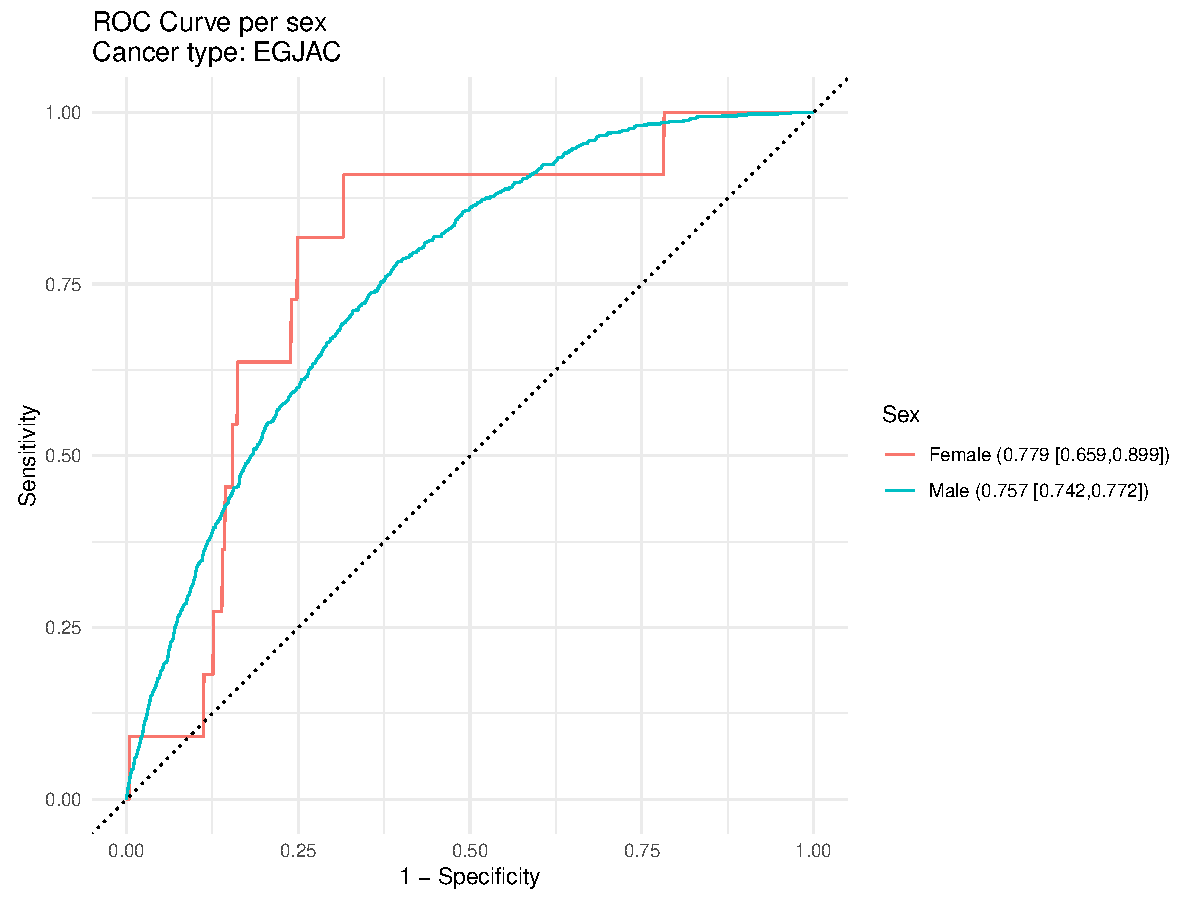
\includegraphics[width=1.0\linewidth]{identity/EGJAC_sex.pdf}
\end{figure}


\newpage
\clearpage
\section{Cancer stage}

\textit{NB: the discrepancy in number of cases between I+ and Any comes from the fact that some were classified as unknown stage according to the provided staging. }


% latex table generated in R 4.2.0 by xtable 1.8-4 package
% Mon Sep 19 18:20:41 2022
\begin{table}[ht]
\centering
\begin{tabular}{lrr}
  \toprule
  \multicolumn{3}{l}{\textbf{ANY}}\\
Stage & Test. AUC & Nb. cases \\ 
  \midrule
Any & 0.799 [0.792,0.807] & 2818 \\ 
   \addlinespace
I & 0.831 [0.815,0.847] & 495 \\ 
  II & 0.813 [0.796,0.831] & 435 \\ 
  III & 0.803 [0.791,0.816] & 878 \\ 
  IV & 0.793 [0.782,0.804] & 1244 \\ 
   \addlinespace
I+ & 0.801 [0.793,0.808] & 2448 \\ 
  II+ & 0.796 [0.788,0.804] & 2169 \\ 
  III+ & 0.794 [0.785,0.803] & 1950 \\ 
  IV+ & 0.793 [0.782,0.804] & 1244 \\ 
   \bottomrule
\end{tabular}
\end{table}
% latex table generated in R 4.2.0 by xtable 1.8-4 package
% Mon Sep 19 14:15:23 2022
\begin{table}[ht]
\centering
\begin{tabular}{lrr}
  \toprule
Stage & Test. AUC & Nb. cases \\ 
  \midrule
Any & 0.796 [0.789,0.803] & 2818 \\ 
   \addlinespace
I & 0.829 [0.813,0.845] & 495 \\ 
  II & 0.810 [0.792,0.828] & 435 \\ 
  III & 0.801 [0.788,0.814] & 878 \\ 
  IV & 0.790 [0.780,0.801] & 1244 \\ 
   \addlinespace
I+ & 0.798 [0.790,0.806] & 2448 \\ 
  II+ & 0.793 [0.785,0.801] & 2169 \\ 
  III+ & 0.791 [0.783,0.800] & 1950 \\ 
  IV+ & 0.790 [0.780,0.801] & 1244 \\ 
   \bottomrule
\end{tabular}
\end{table}

% latex table generated in R 4.2.0 by xtable 1.8-4 package
% Mon Sep 19 14:18:16 2022
\begin{table}[ht]
\centering
\begin{tabular}{lrr}
  \toprule
Stage & Test. AUC & Nb. cases \\ 
  \midrule
Any & 0.773 [0.765,0.780] & 2818 \\ 
   \addlinespace
I & 0.805 [0.789,0.821] & 495 \\ 
  II & 0.789 [0.771,0.808] & 435 \\ 
  III & 0.772 [0.759,0.785] & 878 \\ 
  IV & 0.771 [0.760,0.782] & 1244 \\ 
   \addlinespace
I+ & 0.773 [0.765,0.781] & 2448 \\ 
  II+ & 0.768 [0.760,0.777] & 2169 \\ 
  III+ & 0.767 [0.758,0.776] & 1950 \\ 
  IV+ & 0.771 [0.760,0.782] & 1244 \\ 
   \bottomrule
\end{tabular}
\end{table}







\newpage
\clearpage
\section{Variable importance}

\subsection{Gain VI}

\begin{figure}[ht]
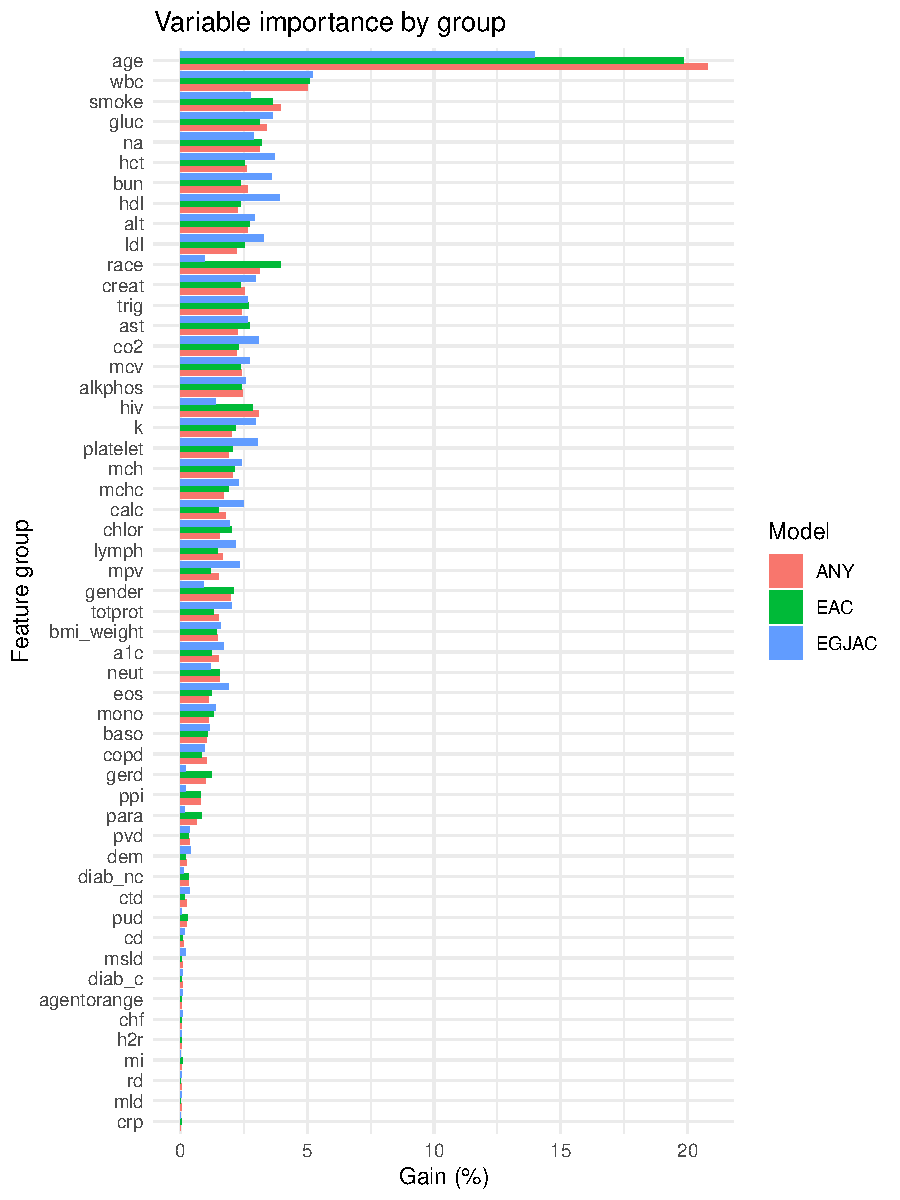
\includegraphics[width=0.8\linewidth]{variable_importance/vi_group.pdf}
\end{figure}

\newpage
\clearpage
\subsection{SHAP VI}


\begin{figure}[ht]
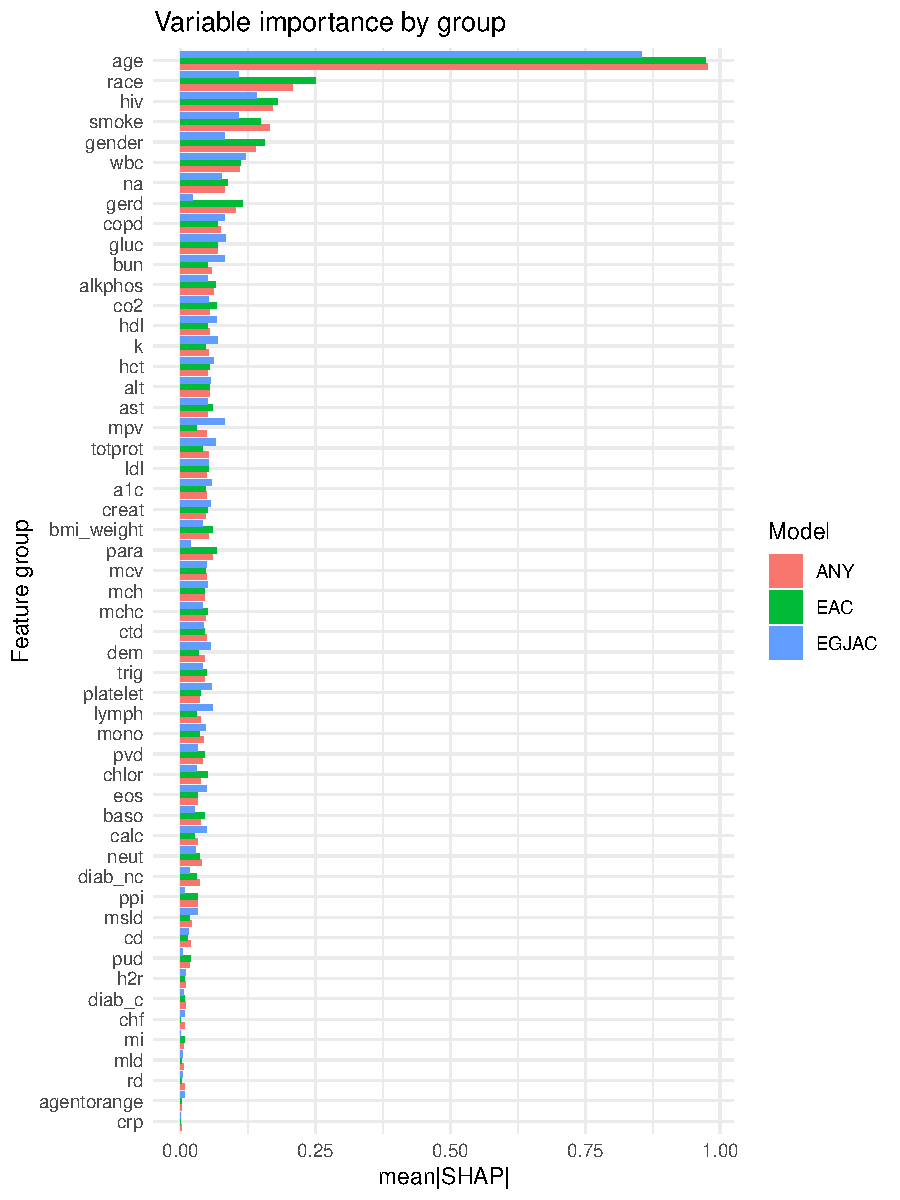
\includegraphics[width=0.8\linewidth]{variable_importance/shap_group.pdf}
\end{figure}





\newpage
\clearpage
\section{Years prior}



\begin{figure}[ht]
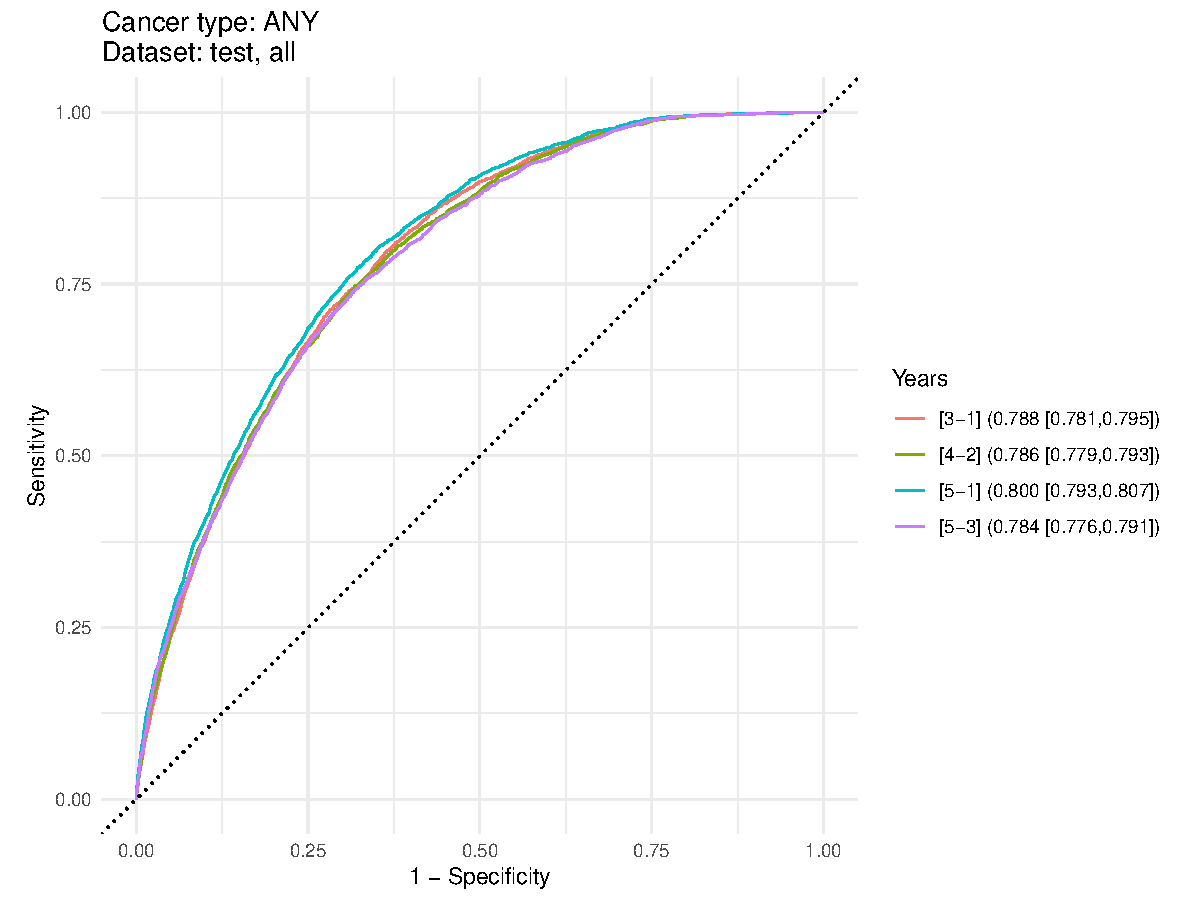
\includegraphics[width=1.0\linewidth]{cancerstage/2y_ANY_all.pdf}
\end{figure}


\begin{figure}[ht]
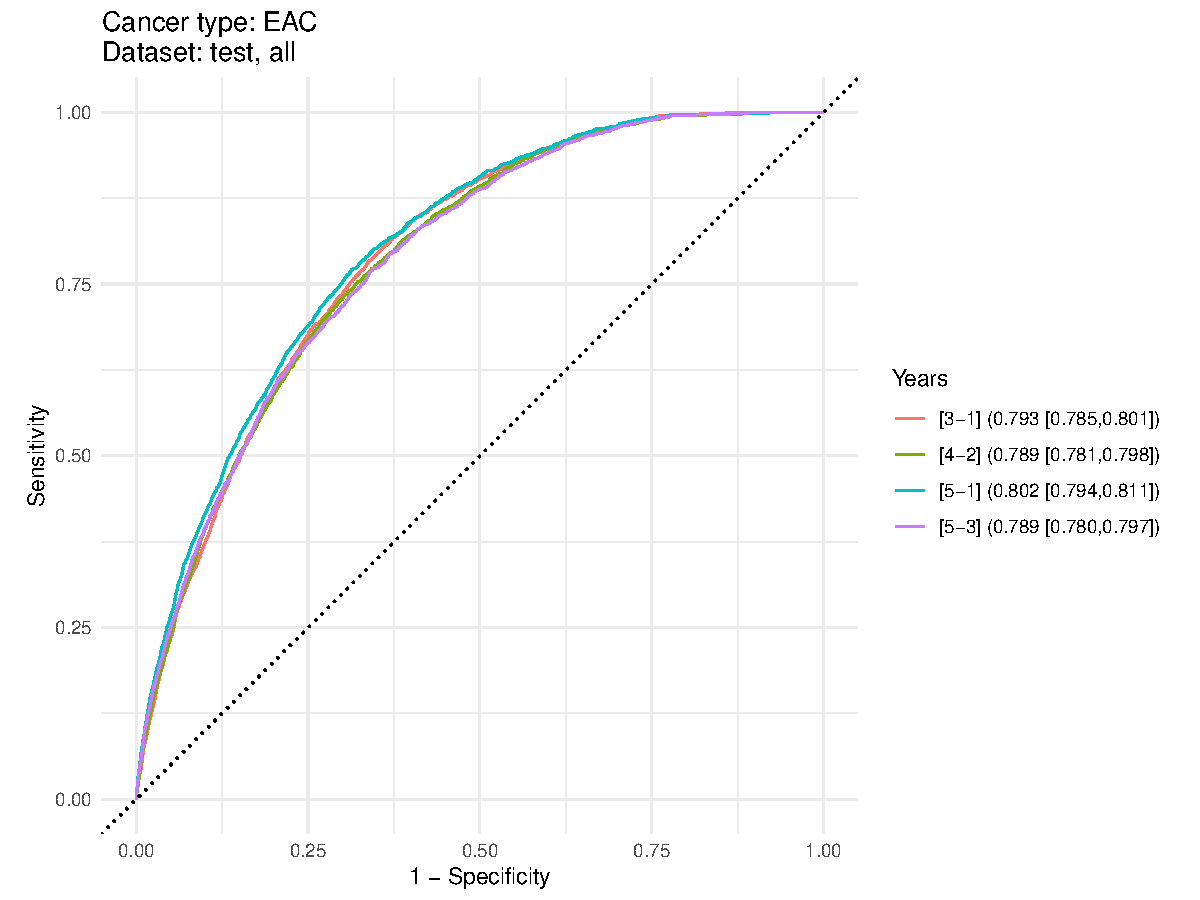
\includegraphics[width=1.0\linewidth]{cancerstage/2y_EAC_all.pdf}
\end{figure}


\begin{figure}[ht]
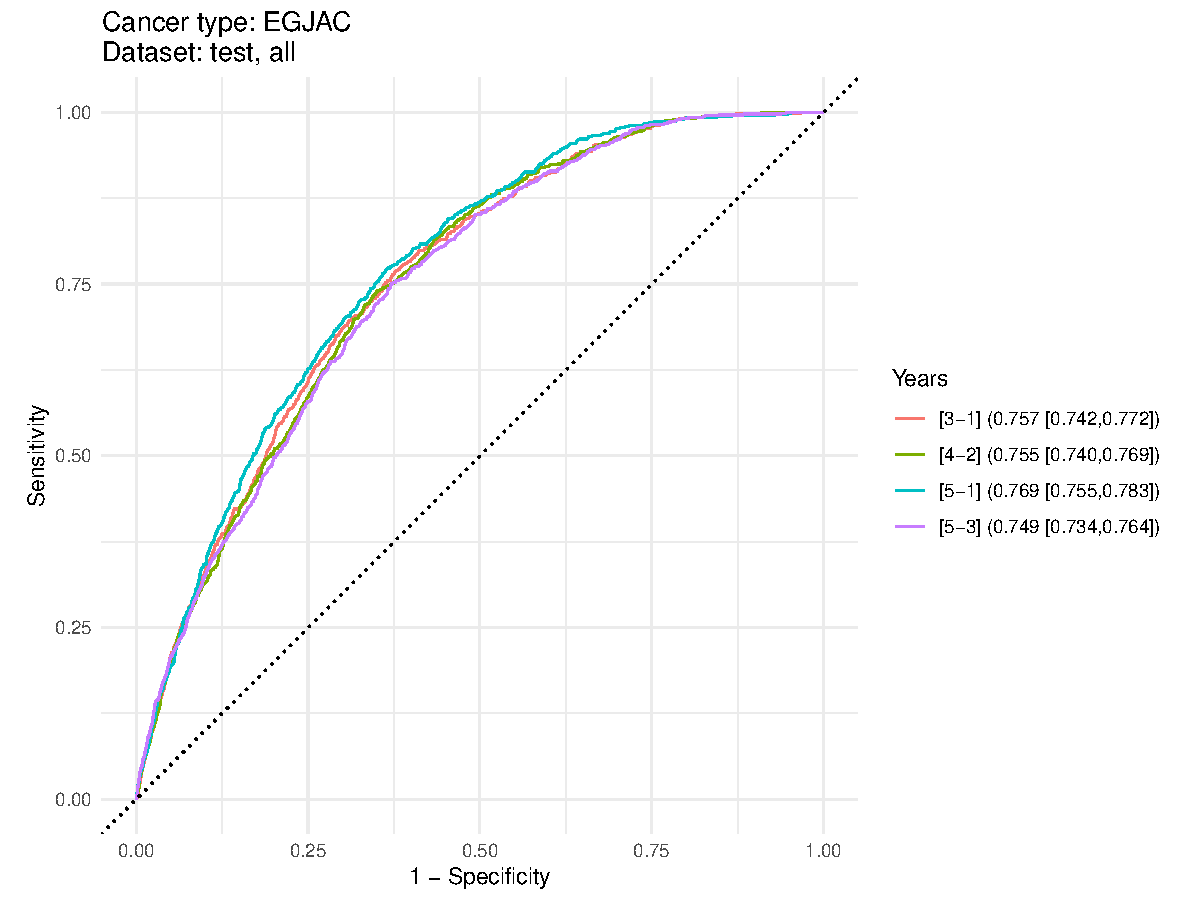
\includegraphics[width=1.0\linewidth]{cancerstage/2y_EGJAC_all.pdf}
\end{figure}




\end{document}
